\section{User Interface (UI)}
The User Interface (UI) of BrainMe is designed with a focus on simplicity, usability, and engagement. We aim to create an intuitive and visually appealing interface that enhances the overall user experience. By adhering to best practices in UI design and incorporating feedback from users, we ensure that the app is both functional and aesthetically pleasing.

\subsection{UI Design Choices}

The UI design choices for BrainMe are centered around creating a seamless and enjoyable user experience. This includes selecting appropriate color schemes, typography, and layout structures that facilitate easy navigation and interaction.

\subsubsection{User Interaction}

User interaction is at the core of BrainMe's design philosophy. The app employs intuitive touch gestures and responsive controls to make it easy for users to navigate through the various features. Buttons, icons, and interactive elements are designed to be easily accessible and recognizable, reducing the learning curve for new users. Feedback mechanisms, such as animations and visual cues, are used to provide immediate responses to user actions, ensuring a smooth and engaging experience.


\subsubsection{Main Design}

The main design of BrainMe is clean and modern, with a focus on clarity and ease of use. The layout is structured to minimize clutter and highlight the most important elements on each screen. Consistent use of colors, fonts, and spacing helps create a cohesive visual experience. The design also incorporates accessibility features, such as adjustable text sizes and high-contrast modes, to ensure that the app is usable by people with diverse needs and preferences.


\subsection{Smartphone UI}

The smartphone UI for BrainMe is optimized for small screens, ensuring that all features are easily accessible and usable on mobile devices. The interface is designed to be responsive, adapting to different screen sizes and orientations to provide a consistent experience across all devices.


\subsubsection{Login and Registration}

The login and registration screens are designed to be simple and straightforward, allowing users to quickly access the app. Clear input fields, helpful instructions, and error messages guide users through the process. Options for signing in with email, Google, or Apple are prominently displayed, making it easy for users to choose their preferred method. The design ensures that users can complete the login or registration process with minimal effort and time.

\begin{figure}[H]
    \centering
    \begin{minipage}[b]{0.43\linewidth}
        \centering
        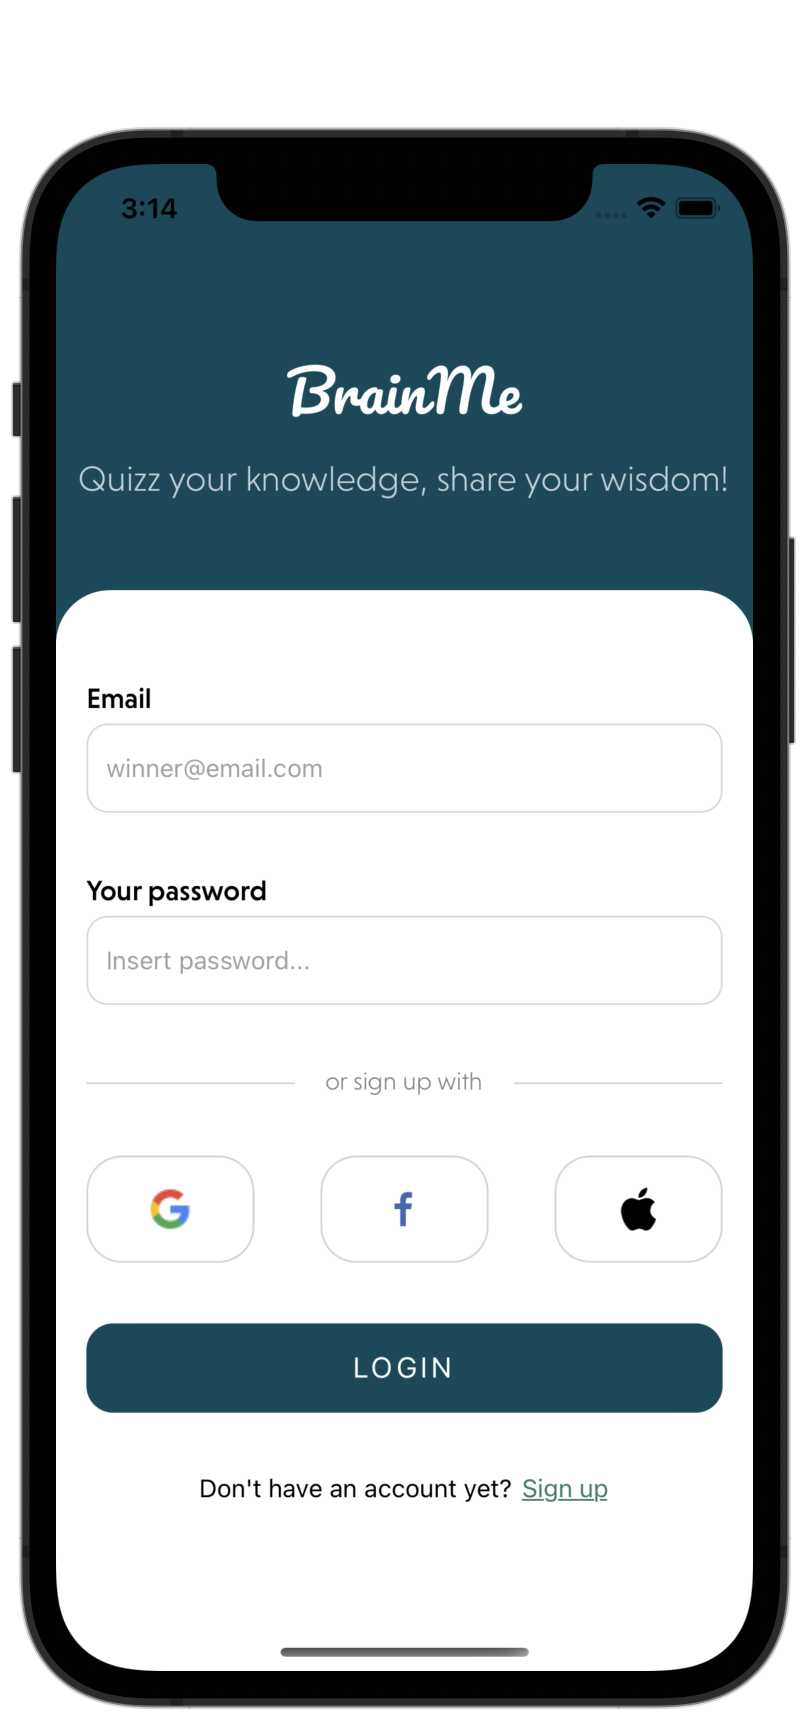
\includegraphics[width=\linewidth]{Mobile UI/Login.png}
        \caption{Login Page}
    \end{minipage}
    \hspace{0.1\linewidth}
    \begin{minipage}[b]{0.43\linewidth}
        \centering
        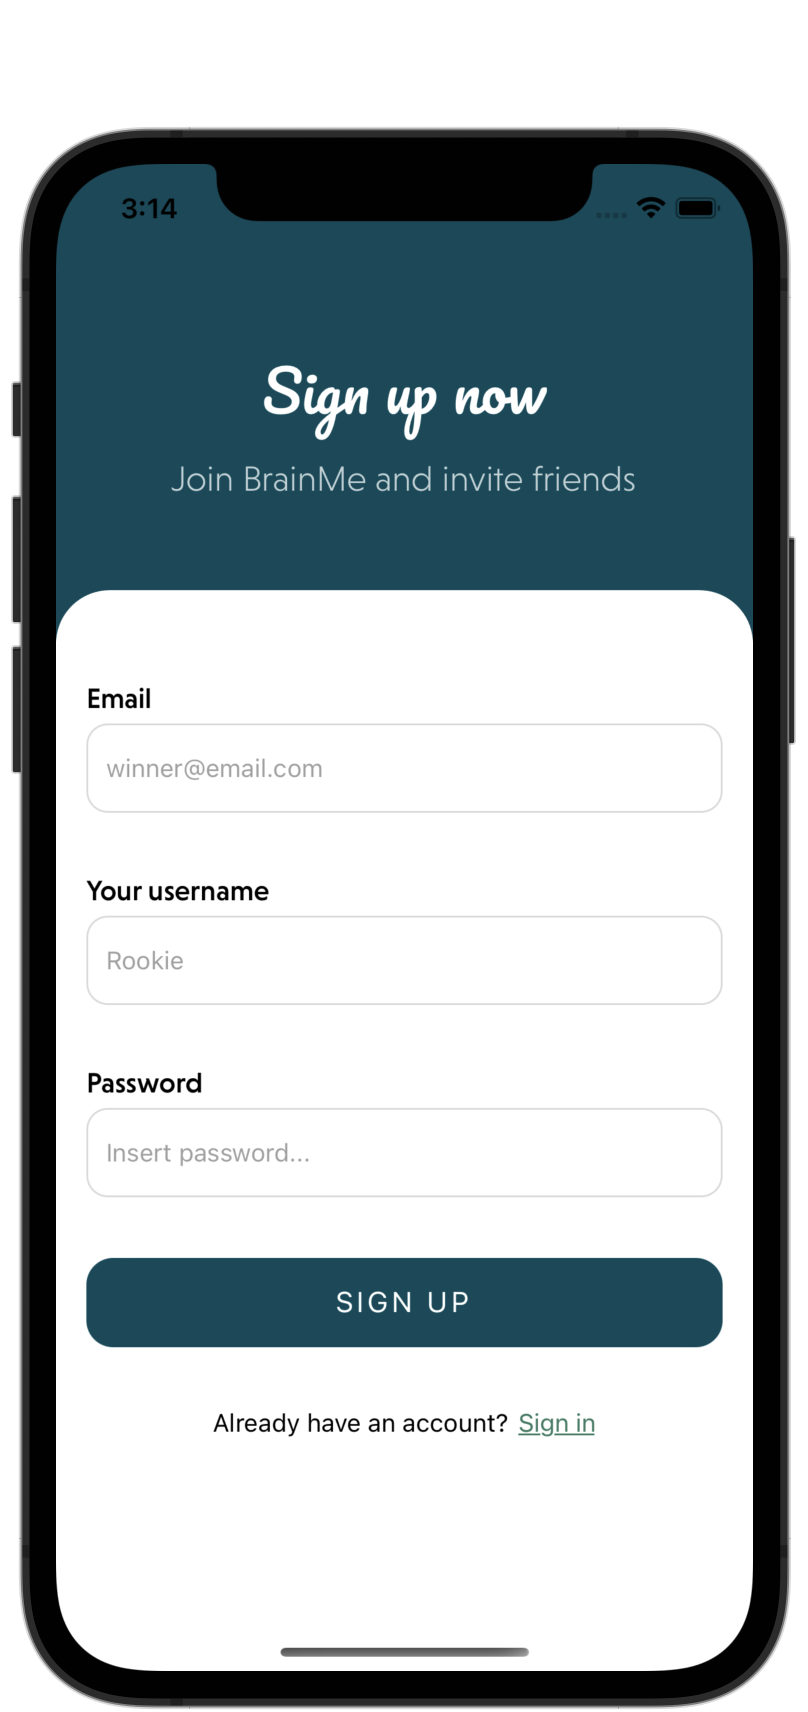
\includegraphics[width=\linewidth]{Mobile UI/Signup.png}
        \caption{Sign Up Page}
    \end{minipage}
    \vspace{0.5cm}
    \caption{\textbf{The BrainMe Application}}
\end{figure}

\subsubsection{Quiz Page: }

The quiz page provides users with a variety of quiz categories to choose from. The interface is designed to be engaging and user-friendly, with clearly labeled icons for each category. Users can easily navigate through different topics such as History, Geography, Music, Arts \& Literature, Science, General Knowledge, Sport, Food, Movie, and Culture. The page also displays the user's current level and progress towards the next level, motivating them to participate in more quizzes. The design ensures that users can quickly select their desired quiz category and start testing their knowledge immediately.

\begin{figure}[H]
    \centering
    \begin{minipage}[b]{0.43\linewidth}
        \centering
        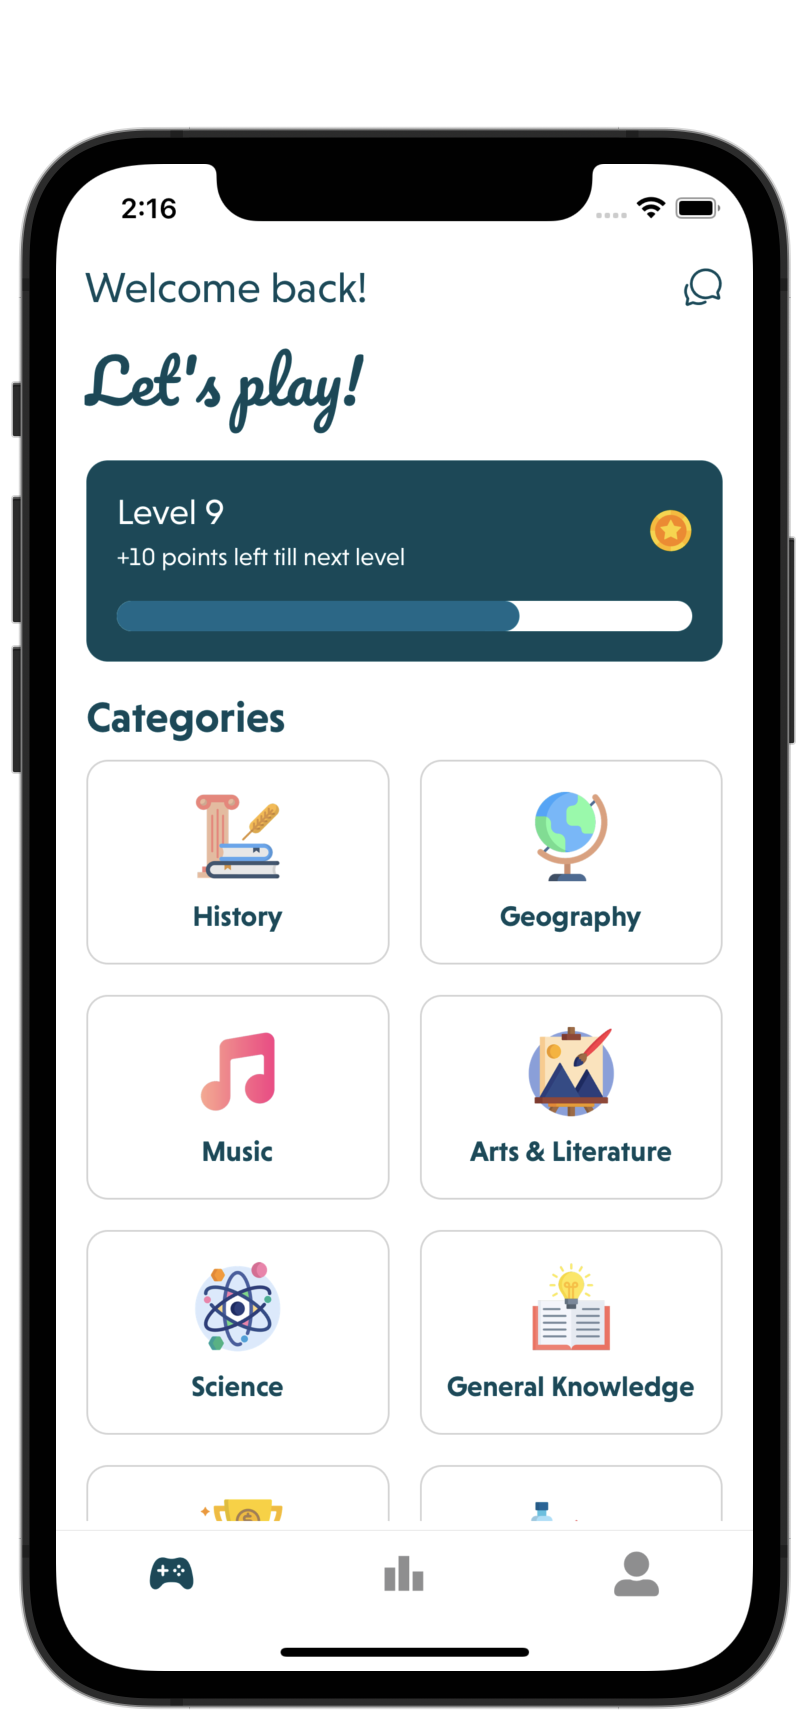
\includegraphics[width=\linewidth]{Mobile UI/Quiz Page 1.png}
        \caption{Quiz Page 1}
    \end{minipage}
    \hspace{0.1\linewidth}
    \begin{minipage}[b]{0.43\linewidth}
        \centering
        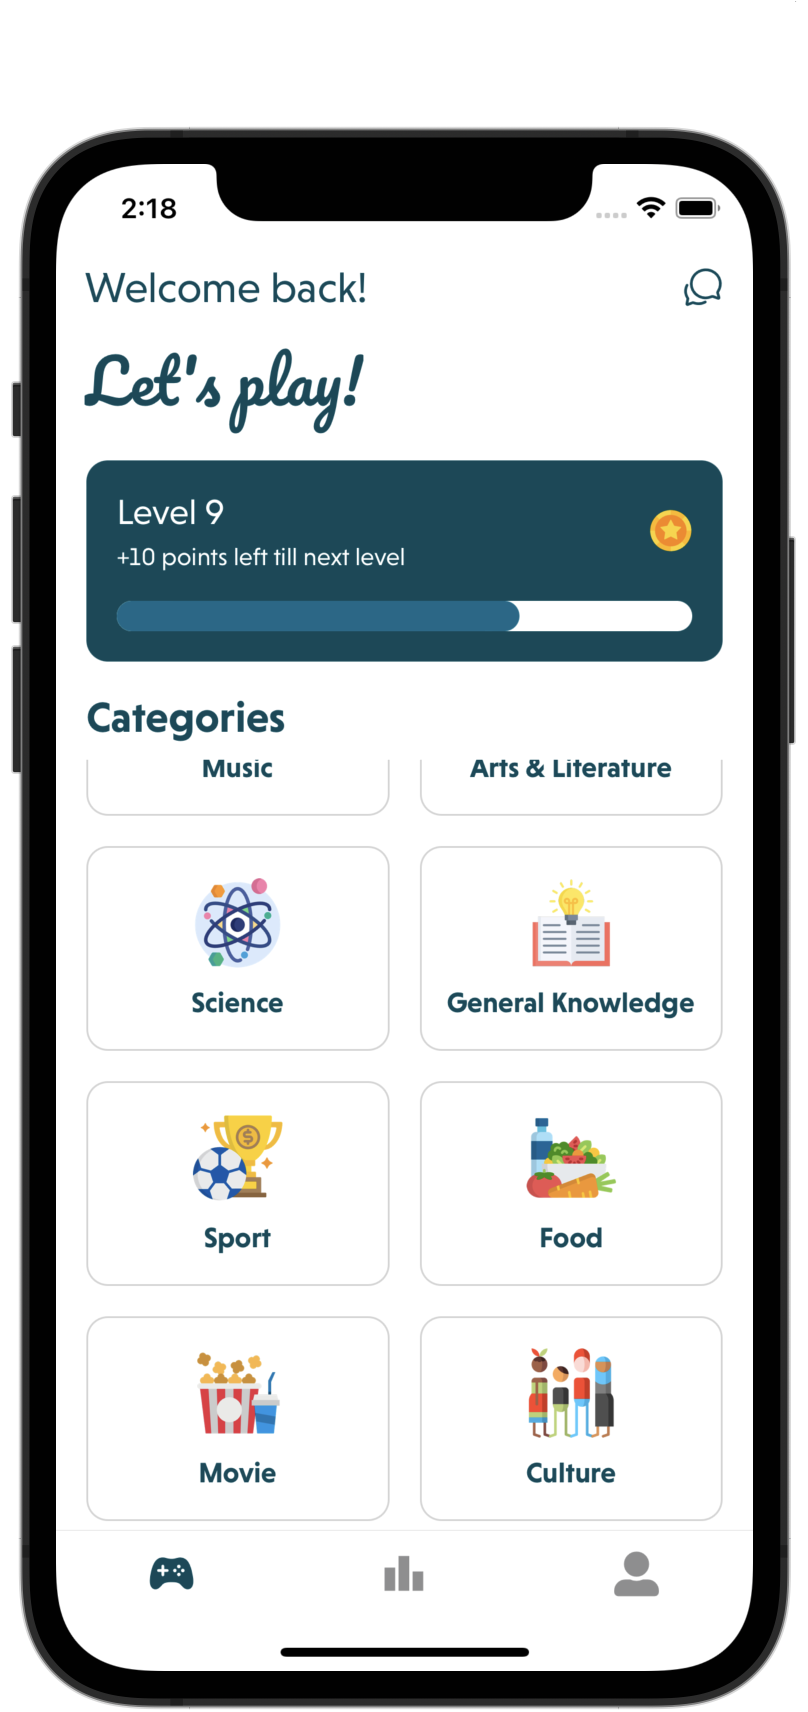
\includegraphics[width=\linewidth]{Mobile UI/Quiz Page 2.png}
        \caption{Quiz Page 2}
    \end{minipage}
    \vspace{0.5cm}
    \caption{\textbf{The BrainMe Application All Quiz Categories}}
\end{figure}


\subsubsection{Quiz Levels: }

The Quiz Levels screen allows users to select the difficulty level of the quiz they want to take. The interface is intuitive, with options for Easy, Medium, and Hard difficulties prominently displayed. Each difficulty level is accompanied by a brief description of what to expect, helping users choose the most suitable challenge. \\\\
The points distribution for each difficulty level is also provided, encouraging users to aim for higher scores by attempting more challenging quizzes. This screen ensures that users are well-informed about their choices and can customize their quiz experience according to their skill level and preferences. \\\\
Lastly, if the user tries to proceed without selecting any difficulty level as in the Figure 21, the user gets to see a message asking to select a difficulty level.

\begin{figure}[H]
    \centering
    \begin{minipage}[b]{0.43\linewidth}
        \centering
        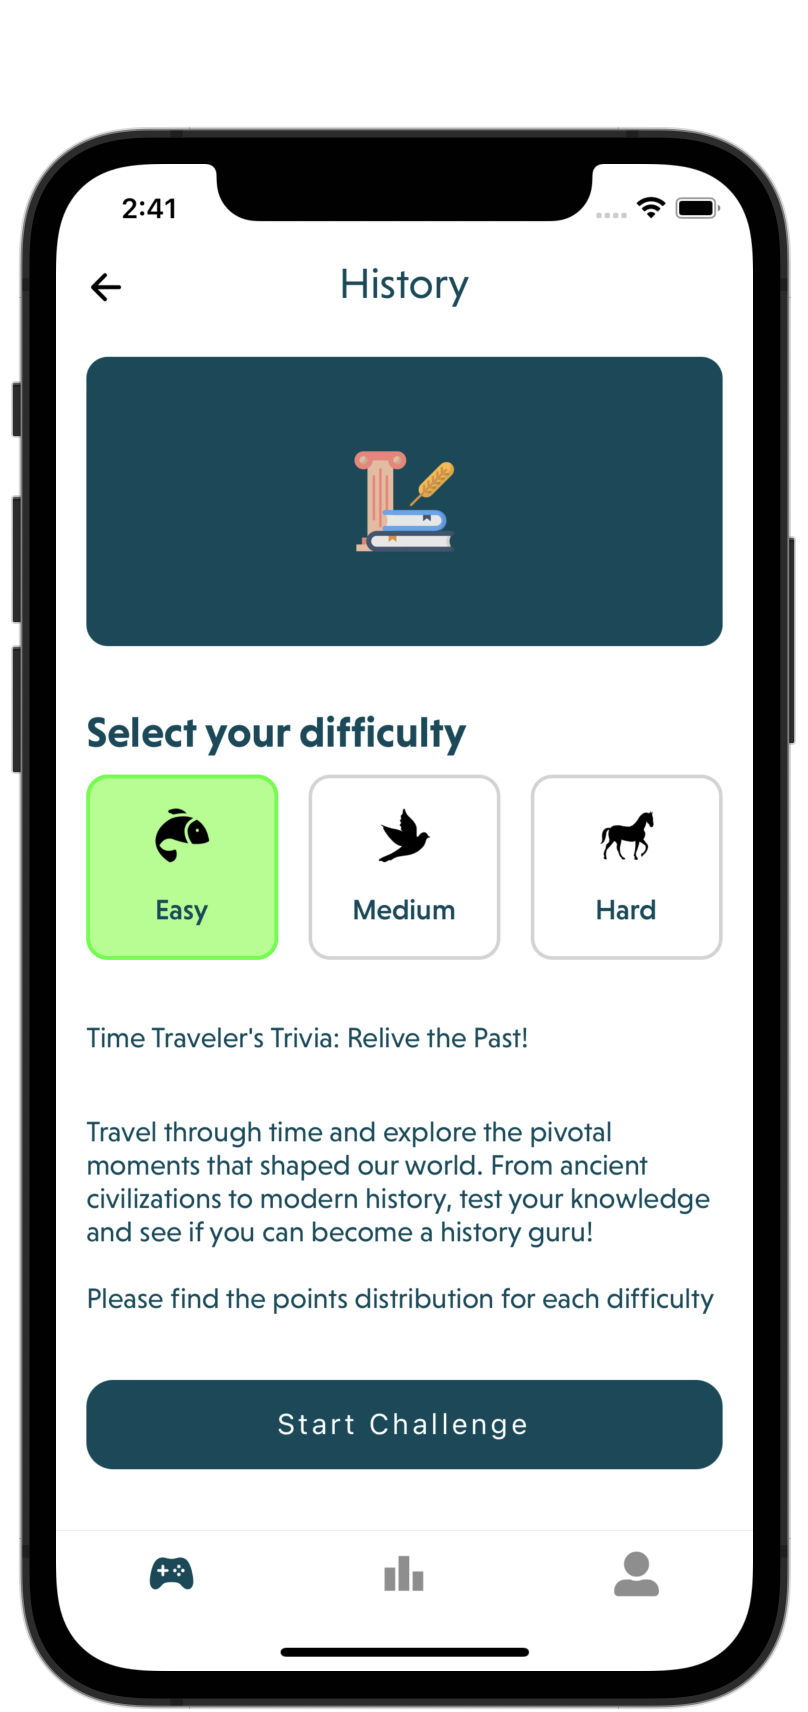
\includegraphics[width=\linewidth]{Mobile UI/Easy Level Quiz.png}
        \caption{Easy Level Quiz}
    \end{minipage}
    \hspace{0.1\linewidth}
    \begin{minipage}[b]{0.43\linewidth}
        \centering
        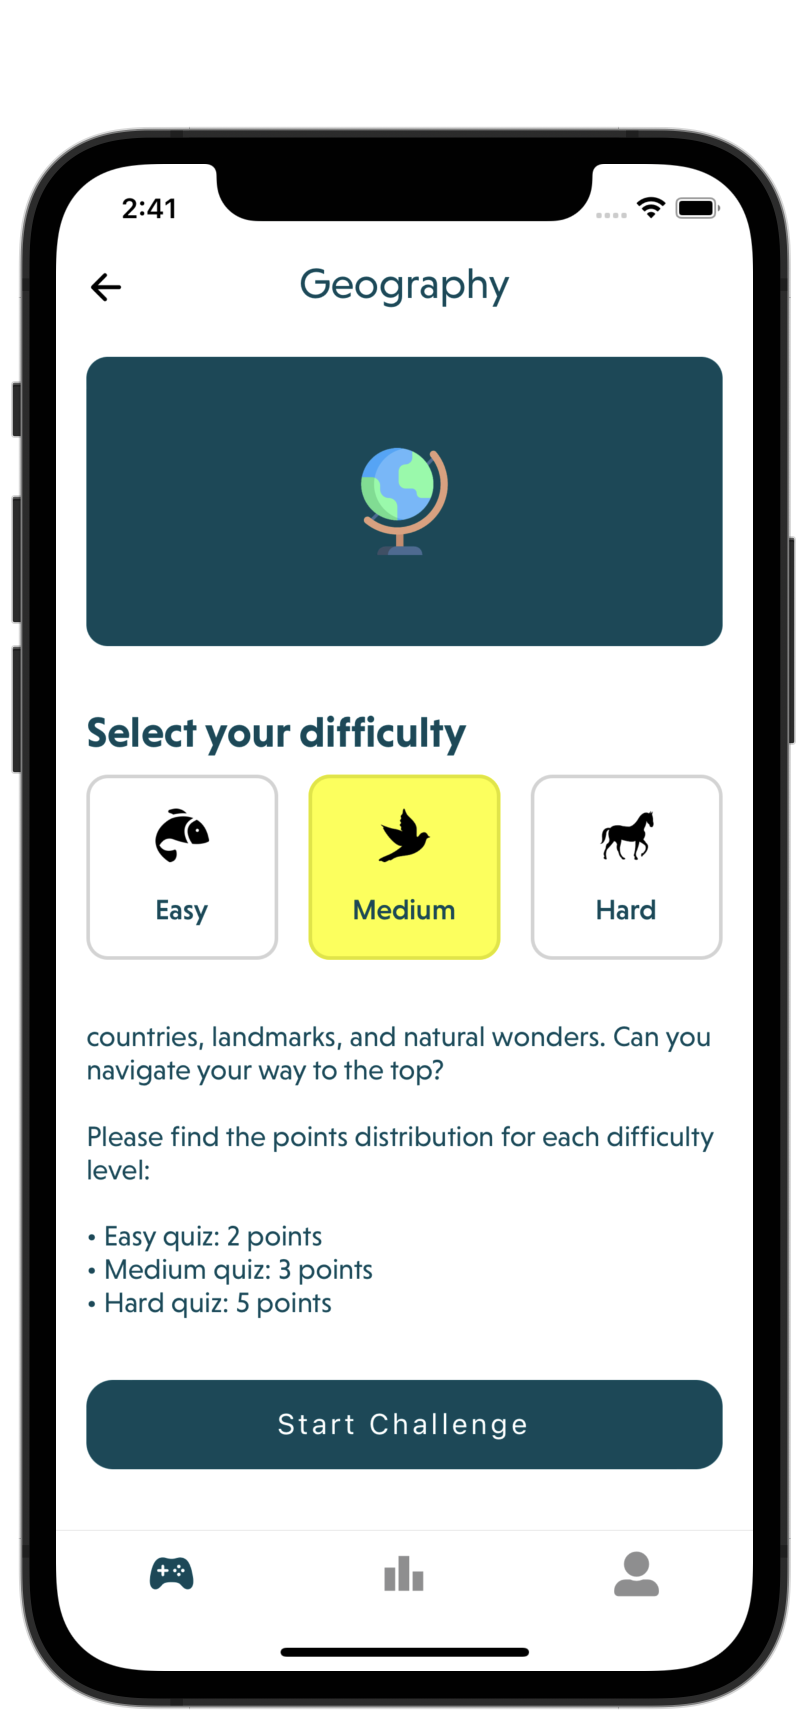
\includegraphics[width=\linewidth]{Mobile UI/Medium Level Quiz.png}
        \caption{Medium Level Quiz}
    \end{minipage}
    \vspace{0.5cm}
    \caption{\textbf{Quiz Difficulty Description}}
\end{figure}


\begin{figure}[H]
    \centering
    \begin{minipage}[b]{0.43\linewidth}
        \centering
        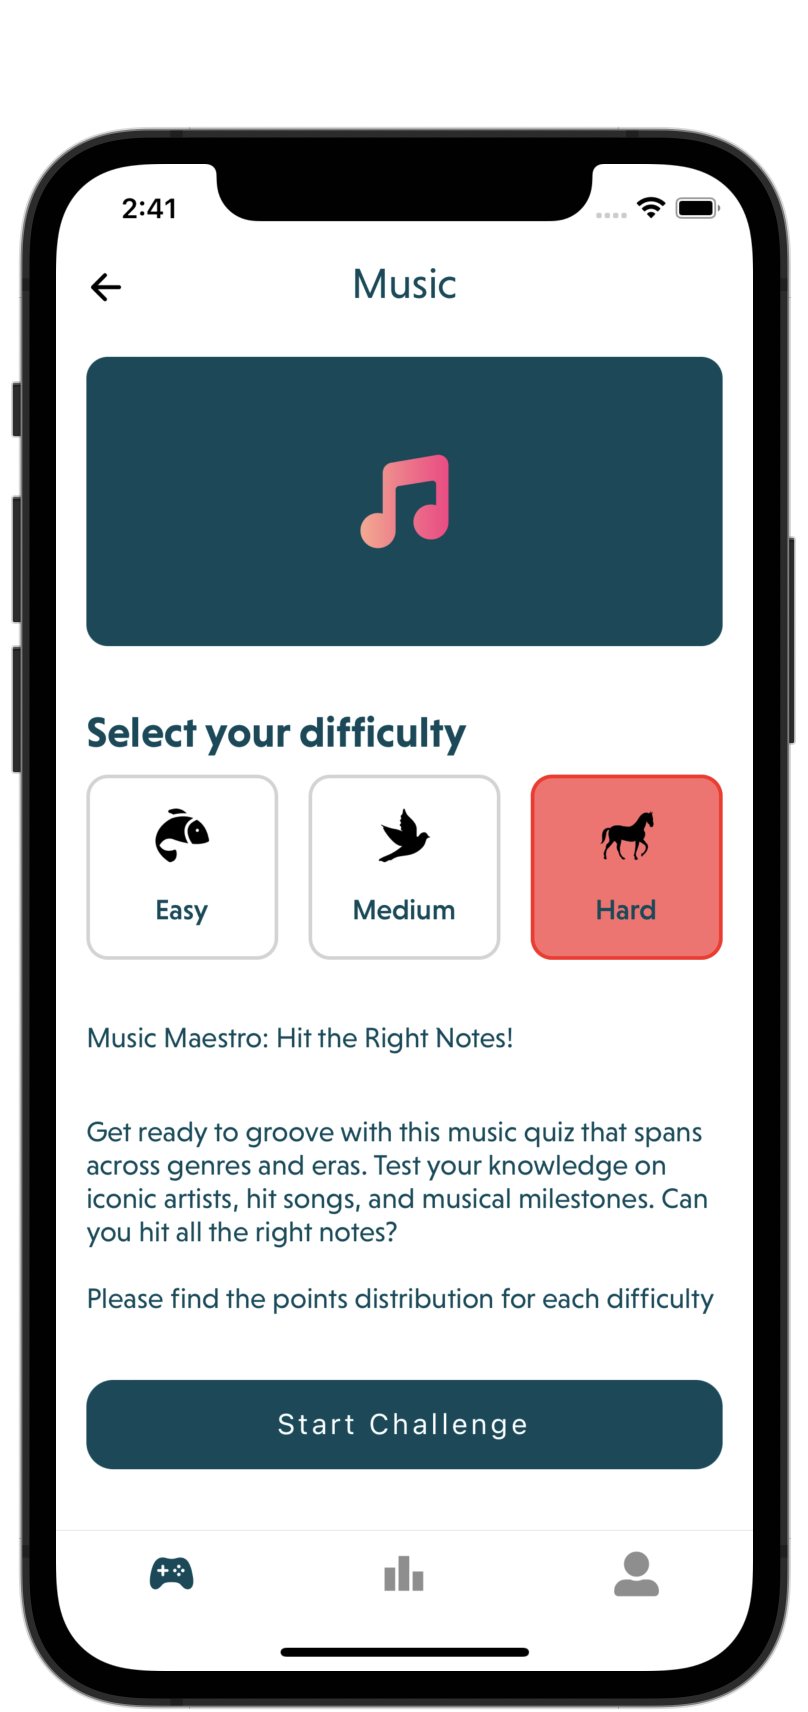
\includegraphics[width=\linewidth]{Mobile UI/Hard Level Quiz.png}
        \caption{Hard Level Quiz}
    \end{minipage}
    \hspace{0.1\linewidth}
    \begin{minipage}[b]{0.43\linewidth}
        \centering
        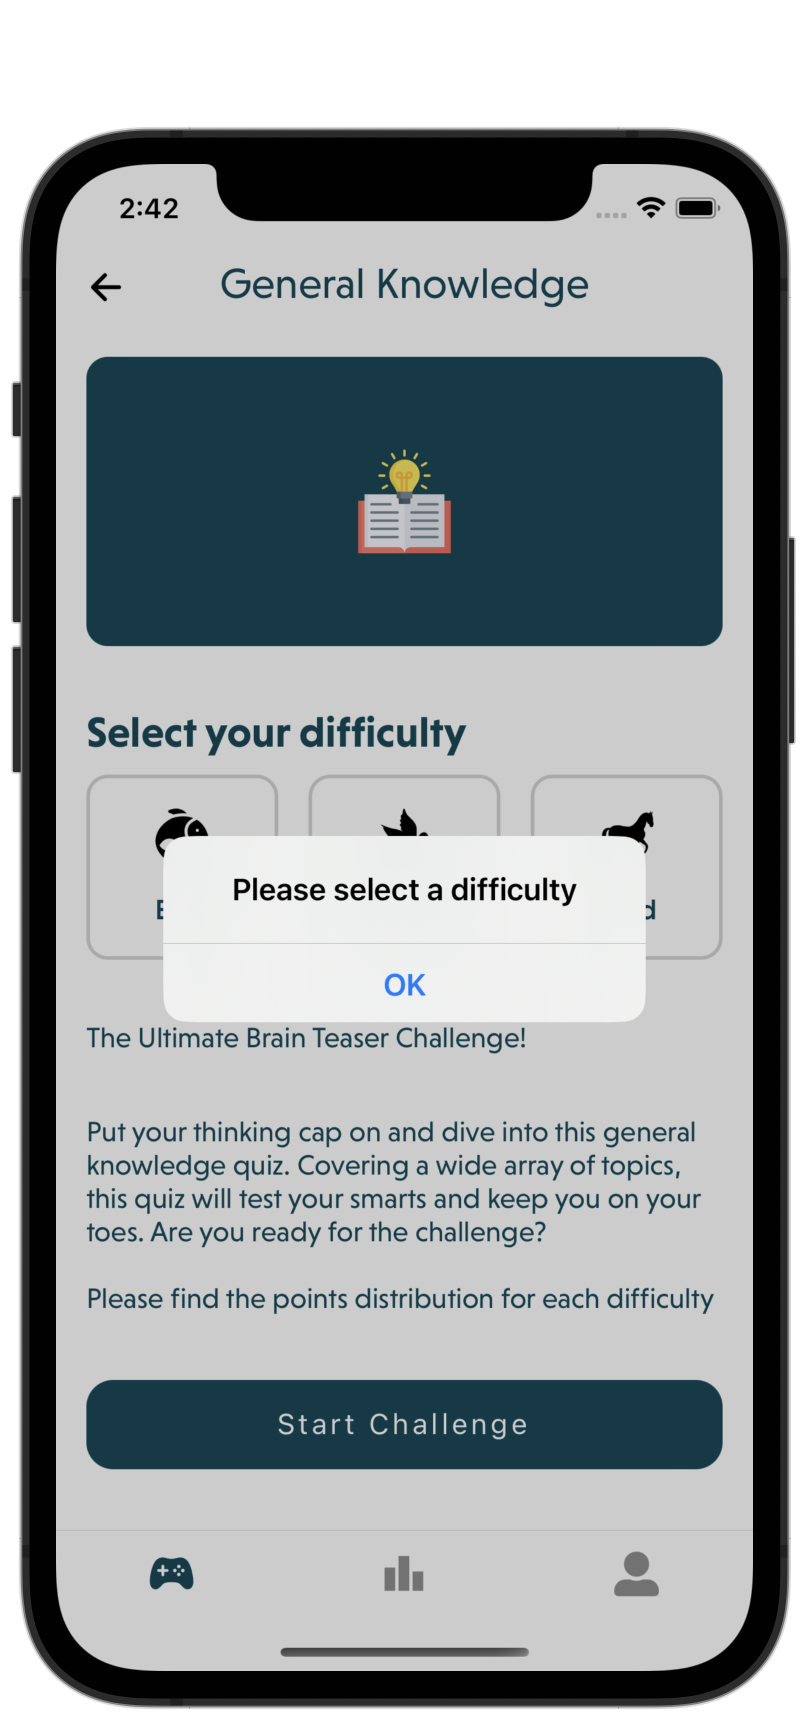
\includegraphics[width=\linewidth]{Mobile UI/Select Difficulty.png}
        \caption{Select Difficulty}
    \end{minipage}
    \vspace{0.5cm}
    \caption{\textbf{Quiz Difficulty Description}}
\end{figure}

\vspace{1cm}

\subsubsection{Starting Quiz}

The starting quiz screens guide users through the process of answering quiz questions. The design ensures that users can easily select their answers and see immediate feedback on their choices.

\begin{figure}[H]
    \centering
    \begin{minipage}[b]{0.43\linewidth}
        \centering
        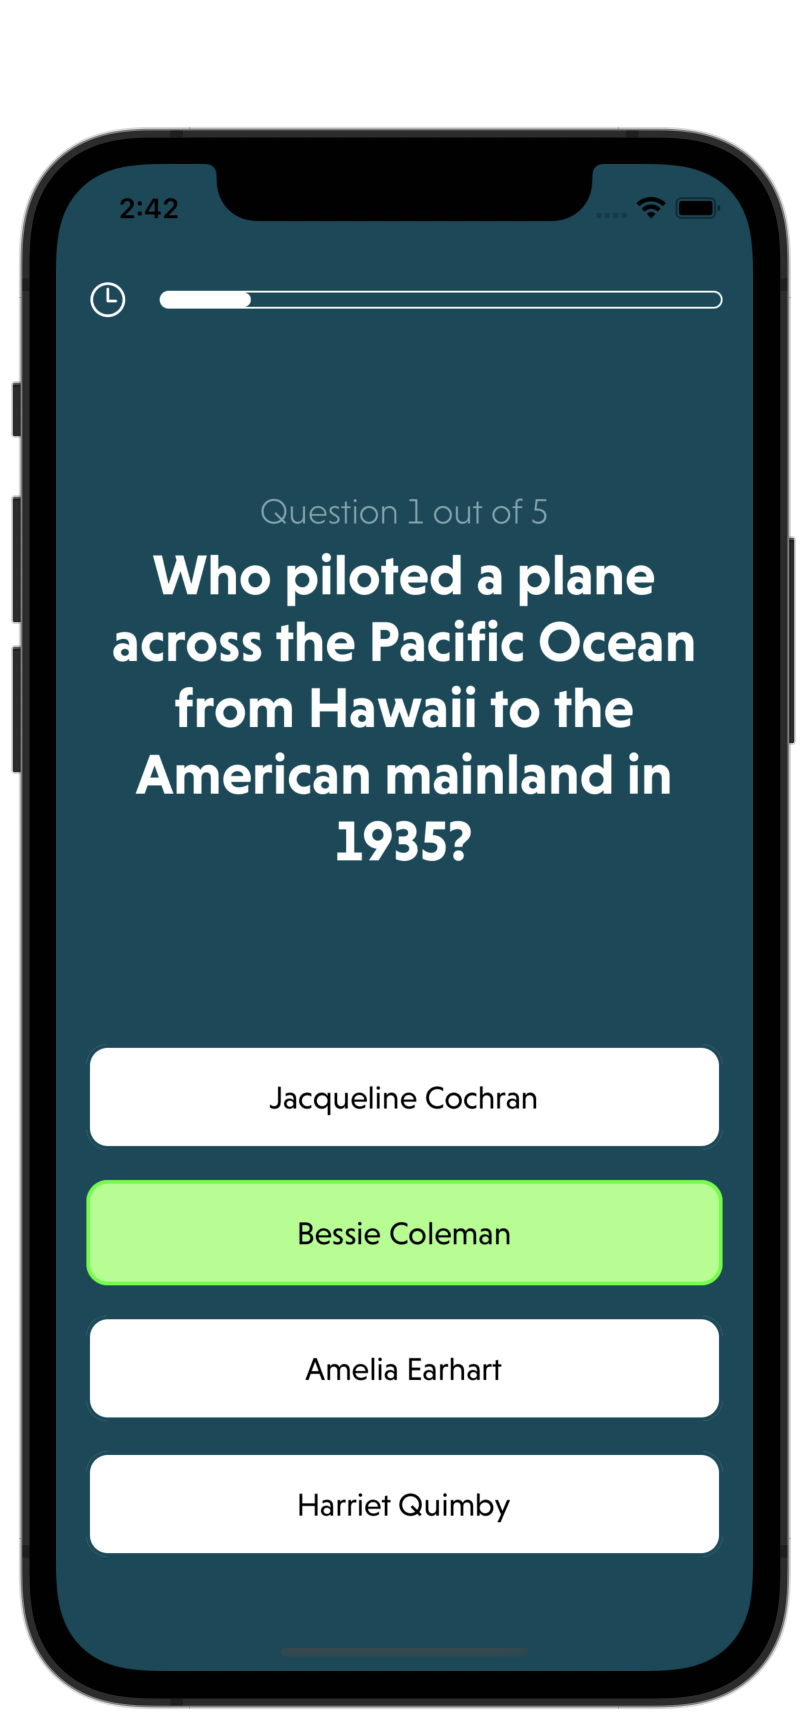
\includegraphics[width=\linewidth]{Mobile UI/User Selecting an option after starting a quiz.png}
        \caption{User selecting an option after starting a quiz}
    \end{minipage}
    \hspace{0.1\linewidth}
    \begin{minipage}[b]{0.43\linewidth}
        \centering
        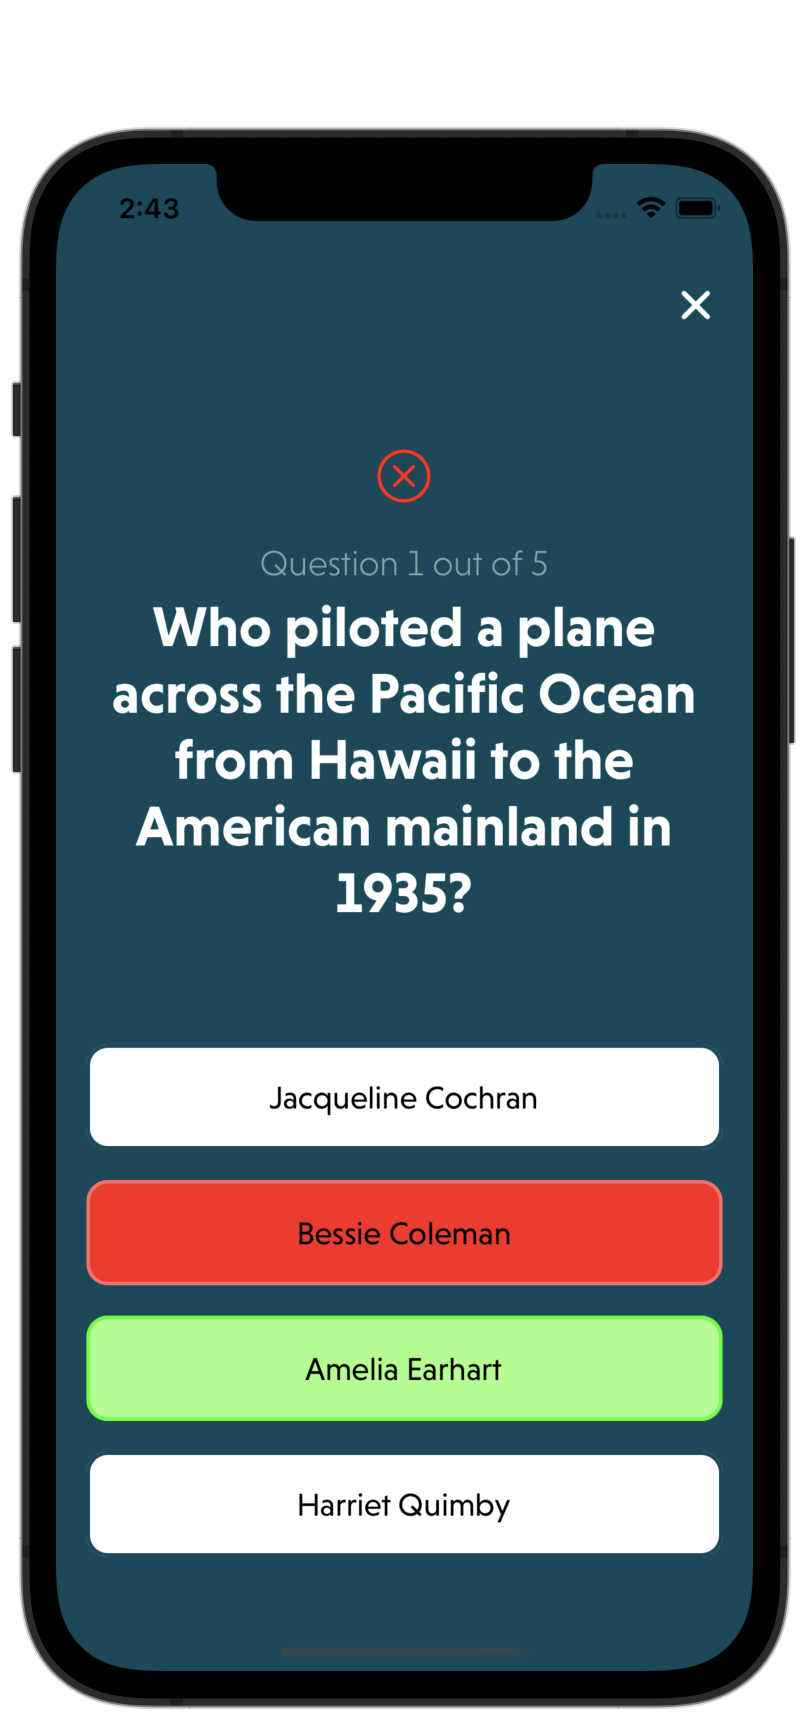
\includegraphics[width=\linewidth]{Mobile UI/Displaying correct result.png}
        \caption{Showing the result after the time has ended}
    \end{minipage}
    \vspace{0.5cm}
    \caption{\textbf{Starting a quiz and selecting an option}}
\end{figure}

\begin{itemize}
    \item The user begins the quiz by selecting a category and difficulty level.
    \item Each question is displayed one at a time, with multiple answer options provided below the question.
    \item When the user selects an option, it is highlighted to indicate their choice (Figure 23).
    \item Once the user submits their answer or the timer runs out, the correct answer is displayed:
    \begin{itemize}
        \item Correct answers are highlighted in green.
        \item Incorrect answers are highlighted in red (Figure 24).
        \item If the user did not select an answer, a message indicating "Did not select" is displayed, and then the correct answer is shown.
    \end{itemize}
    \item This immediate feedback helps users understand their mistakes and learn the correct information right away.
\end{itemize}

\vspace{1cm}

\subsubsection{Ending and Reviewing Quiz}

The ending and reviewing quiz screens provide users with a summary of their performance and an option to review their answers. These screens are designed to help users understand their mistakes and learn from them, enhancing the overall learning experience.

\begin{itemize}
    \item After completing a quiz, the user is presented with the quiz results screen.
    \item The quiz results screen displays the total number of questions, correct answers, and wrong answers.
    \item The user has the option to review their answers by tapping the "Review Answers" button.
    \item If the user chooses to review their answers:
    \begin{itemize}
        \item The quiz review screen displays each question along with the user's selected answer and the correct answer.
        \item Correct answers are highlighted in green icon, while incorrect answers are highlighted in red icon.
    \end{itemize}
    \item The user can also choose to return to the home page by tapping the "Return Home" button.
\end{itemize}

\begin{figure}[H]
    \centering
    \begin{minipage}[b]{0.43\linewidth}
        \centering
        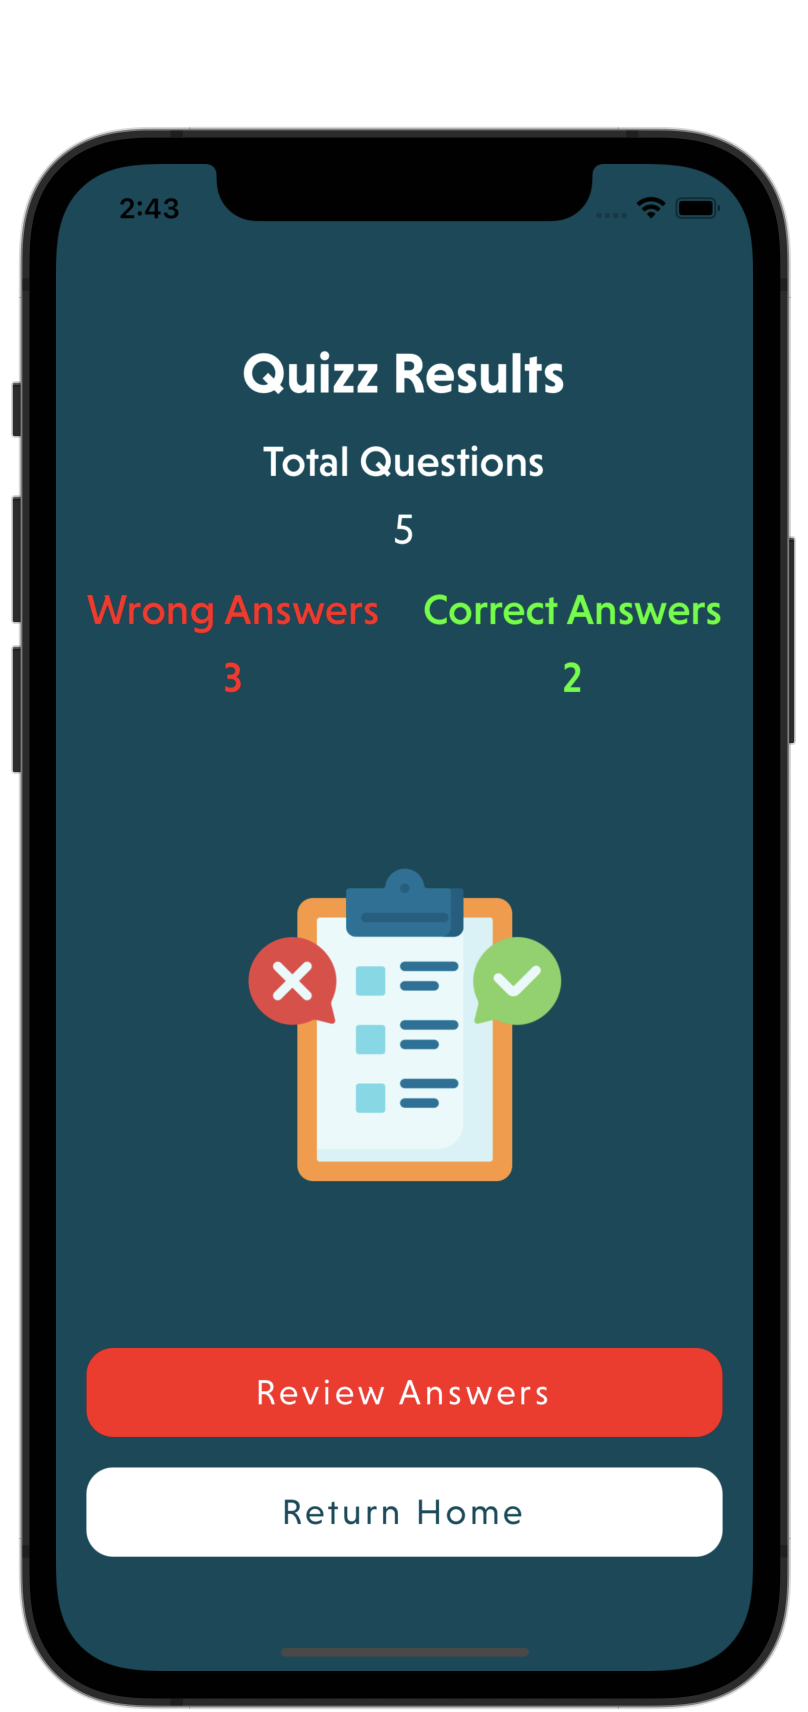
\includegraphics[width=\linewidth]{Mobile UI/Quiz Result.png}
        \caption{Quiz Results with options to review or return home}
    \end{minipage}
    \hspace{0.1\linewidth}
    \begin{minipage}[b]{0.43\linewidth}
        \centering
        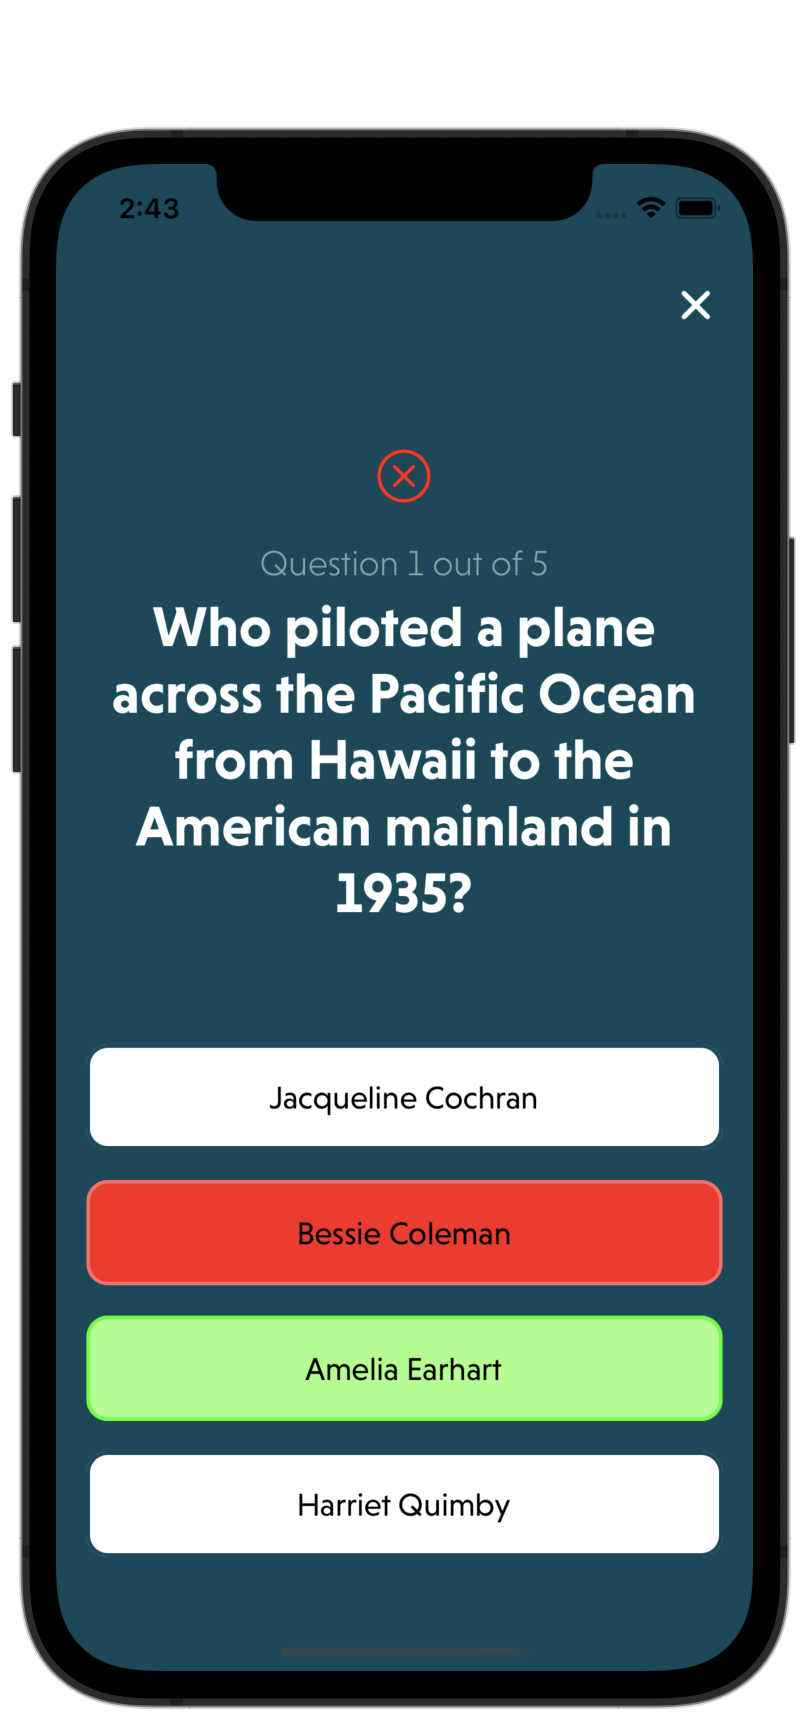
\includegraphics[width=\linewidth]{Mobile UI/Displaying correct result.png}
        \caption{Displaying correct result for incorrect solution}
    \end{minipage}
    \vspace{0.5cm}
    \caption{\textbf{Ending a quiz and selecting an option}}
\end{figure}


\begin{figure}[H]
    \centering
    \begin{minipage}[b]{0.43\linewidth}
        \centering
        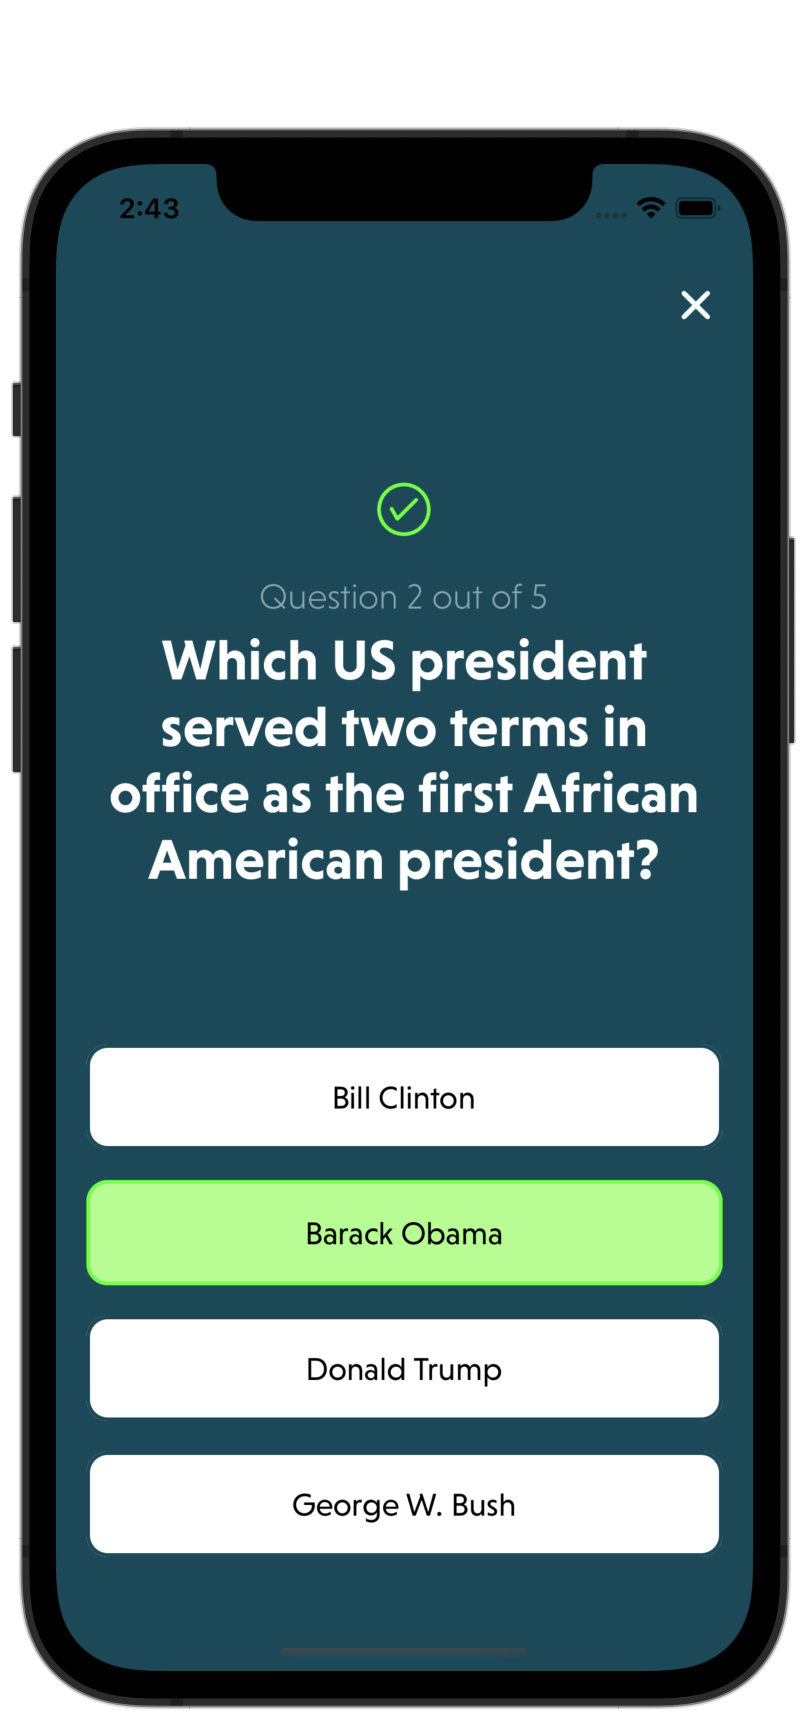
\includegraphics[width=\linewidth]{Mobile UI/Reviewing correct solution.png}
        \caption{Reviewing correct solution for correct selection}
    \end{minipage}
    \hspace{0.1\linewidth}
    \begin{minipage}[b]{0.43\linewidth}
        \centering
        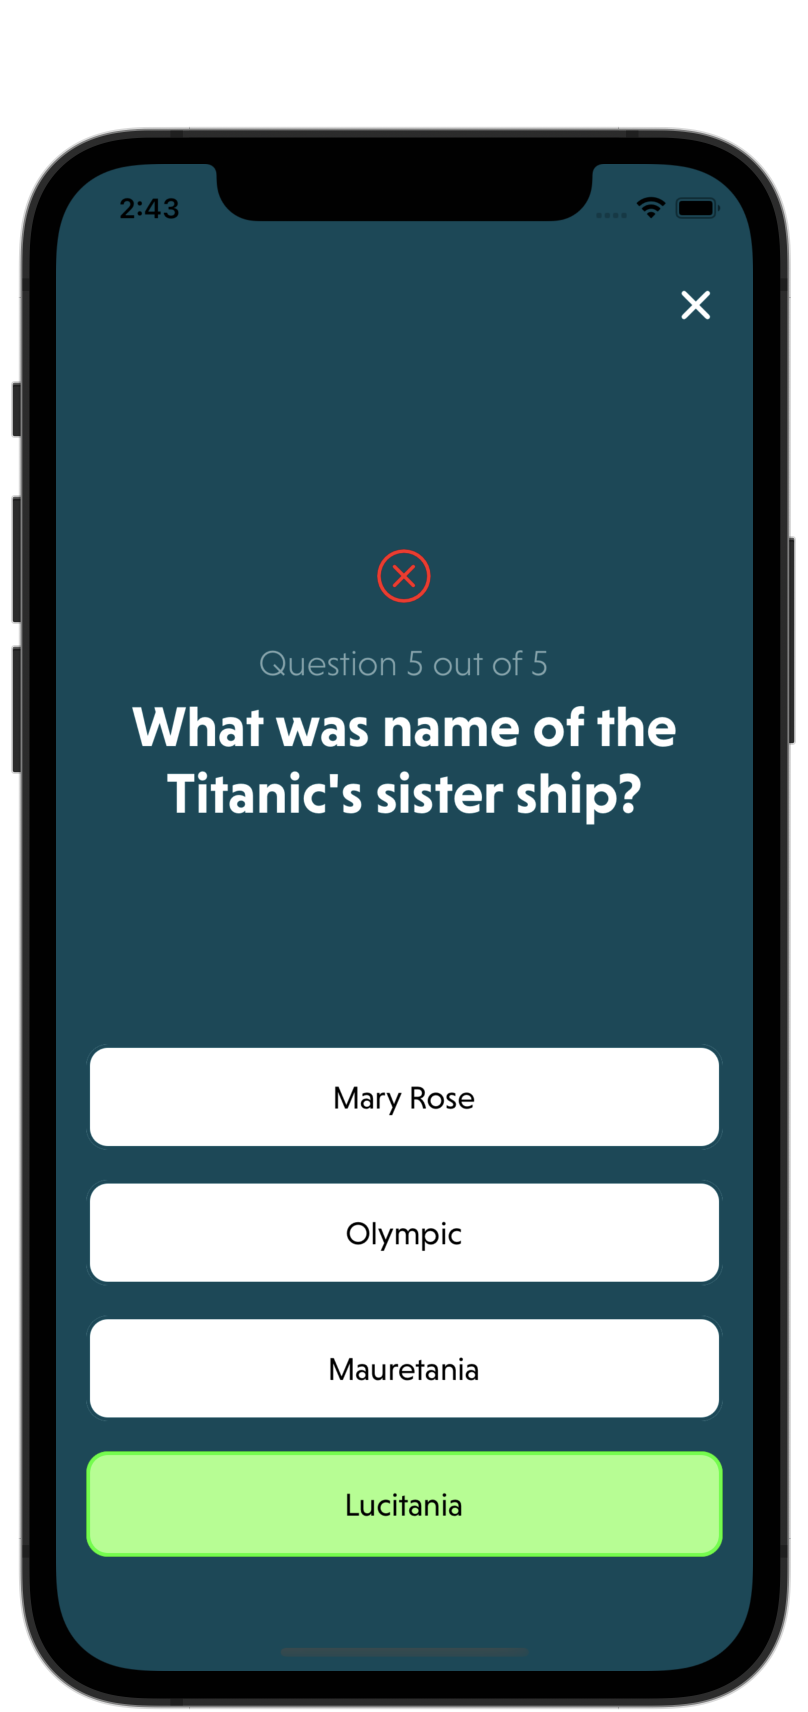
\includegraphics[width=\linewidth]{Mobile UI/Result when no selection has been made.png}
        \caption{Reviewing correct solution for no selection}
    \end{minipage}
    \vspace{0.5cm}
    \caption{\textbf{Reviewing the correct result}}
\end{figure}

\subsubsection{Leaderboard}

The leaderboard feature in the BrainMe application displays the ranking of users based on their quiz performance. This promotes a competitive environment, motivating users to improve their scores and climb the ranks. Users can view their position relative to others, fostering a sense of achievement and encouraging active participation in quizzes.

\begin{figure}[H]
    \centering
    \begin{minipage}[b]{0.3\linewidth}
        \centering
        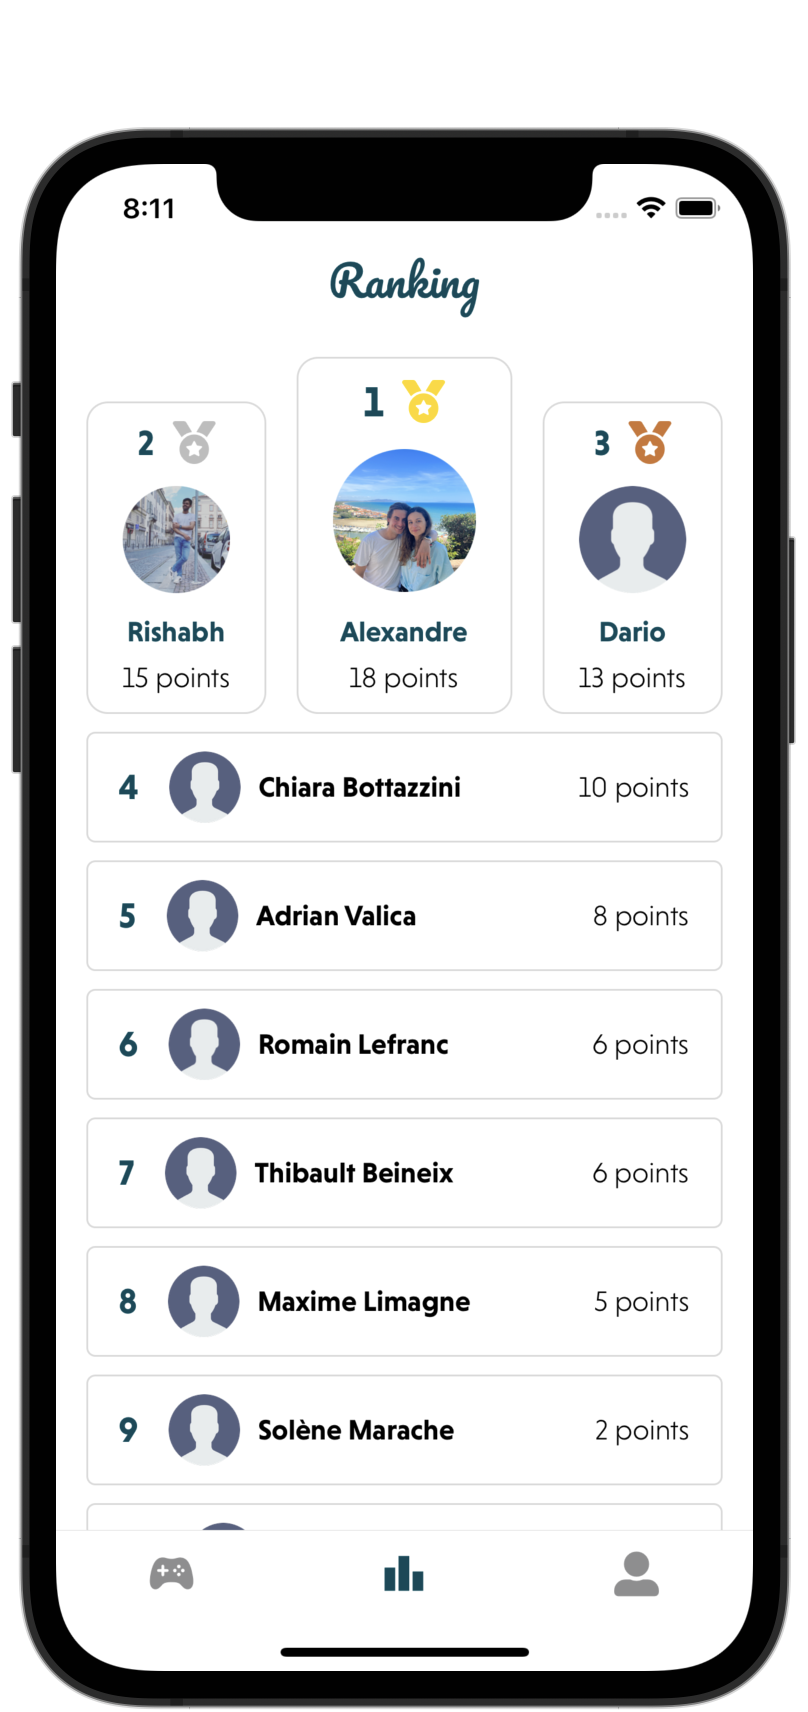
\includegraphics[width=\linewidth]{Mobile UI/Initial Leaderboard.png}
        \caption{Leaderboard ranking depicting medals and rankings}
    \end{minipage}
    \hspace{0.02\linewidth}
    \begin{minipage}[b]{0.3\linewidth}
        \centering
        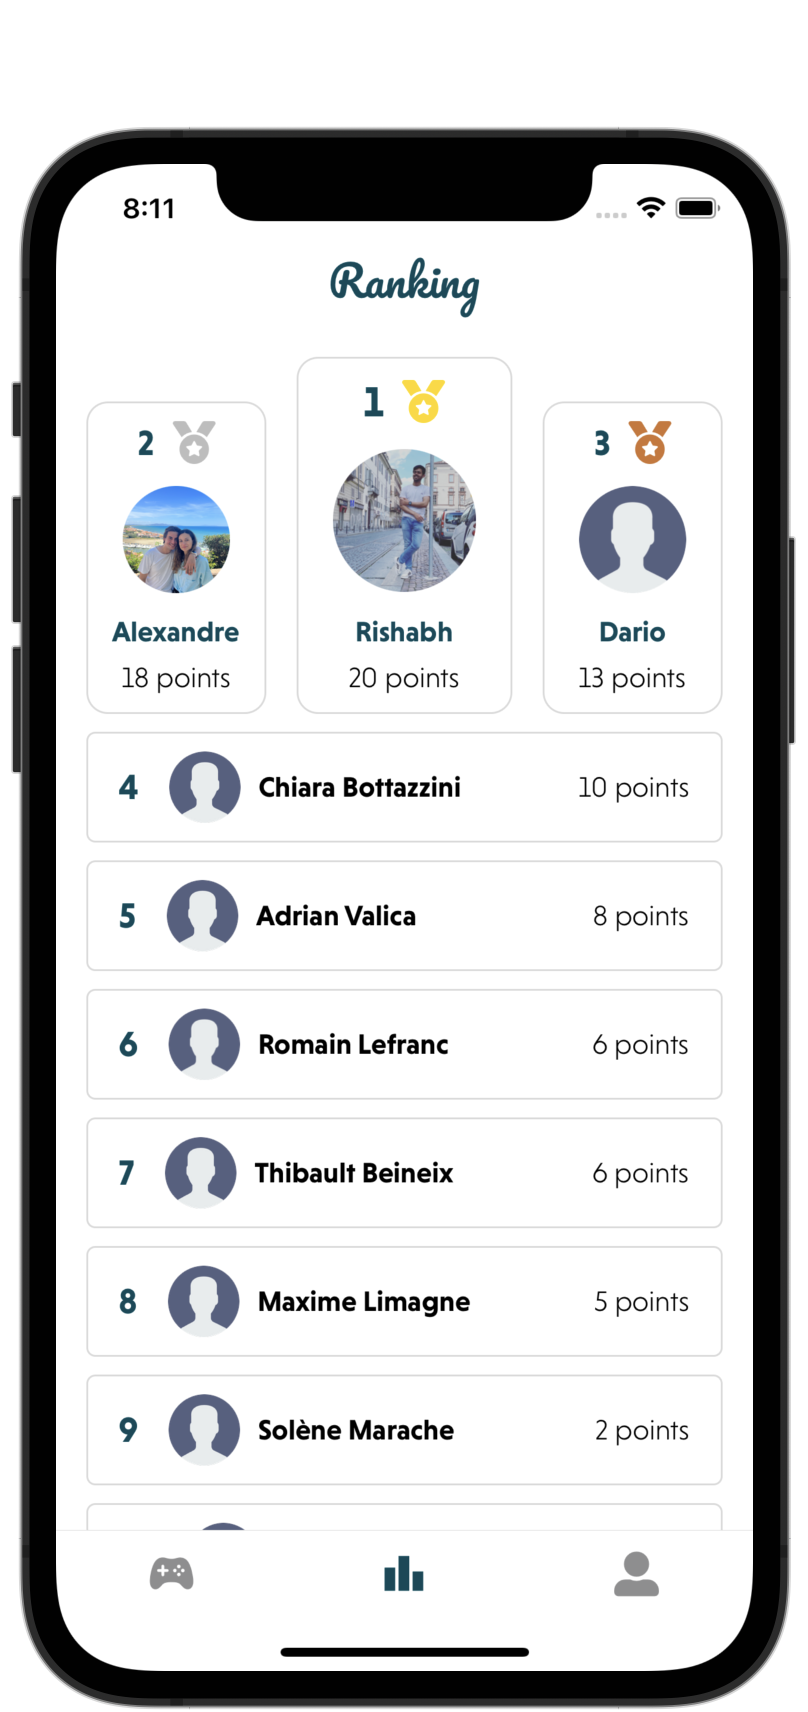
\includegraphics[width=\linewidth]{Mobile UI/Final Leaderboard.png}
        \caption{Change in leaderboard position from second to first}
    \end{minipage}
    \hspace{0.02\linewidth}
    \begin{minipage}[b]{0.3\linewidth}
        \centering
        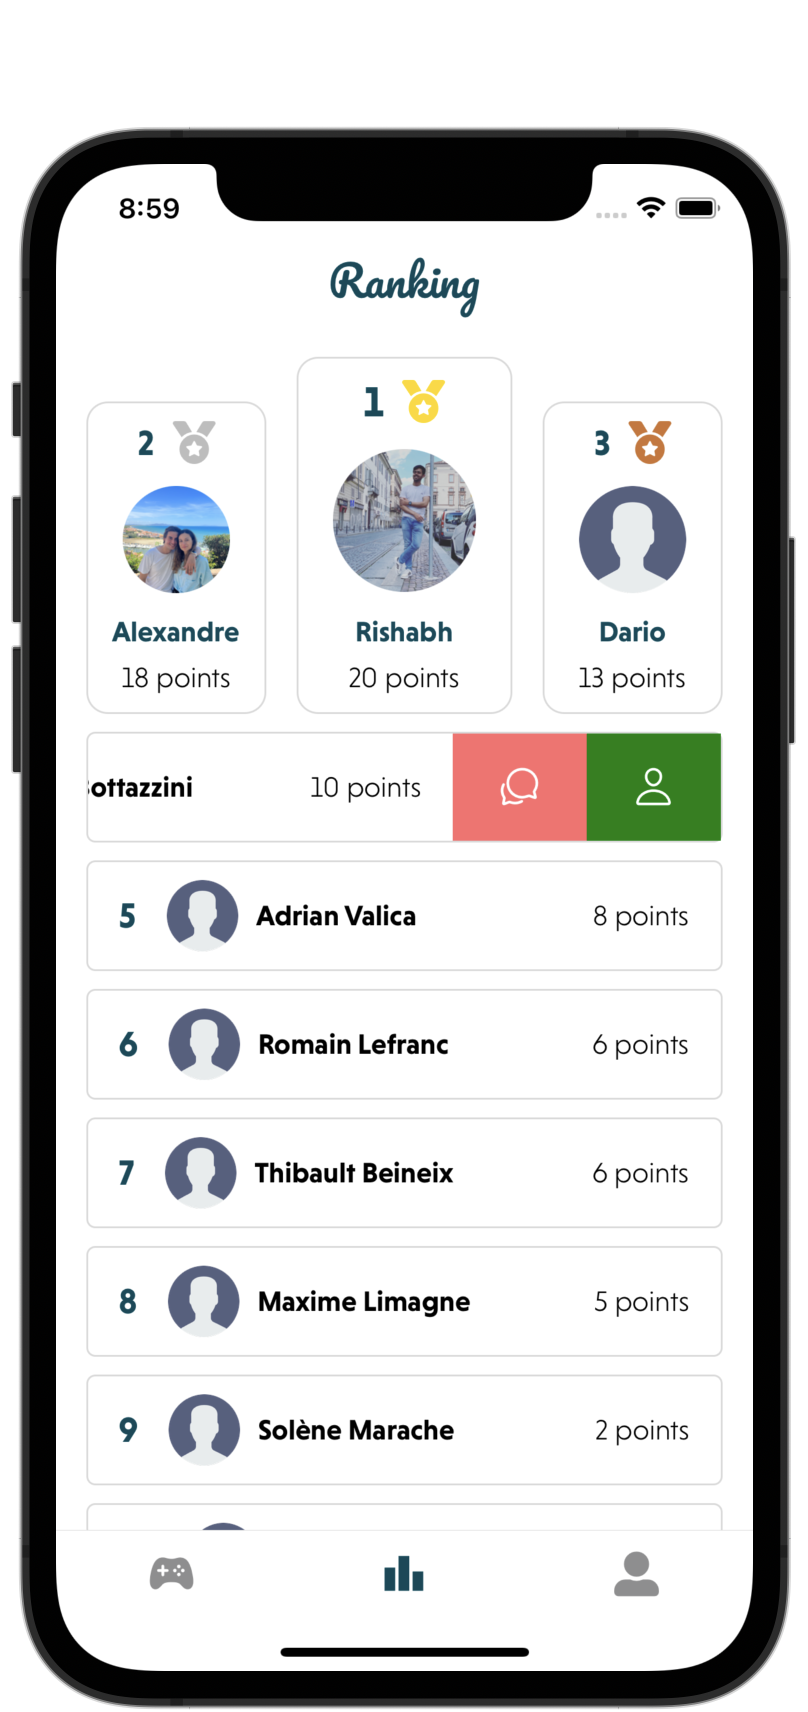
\includegraphics[width=\linewidth]{leaderboard chat.png}
        \caption{Sliding on the name to chat or view profile}
    \end{minipage}
    \vspace{0.5cm}
    \caption{\textbf{Depicting a change in the position of leaderboard ranking and the medals along with chat option}}
\end{figure}


\begin{itemize}
\item \textbf{Real-time updates:} The leaderboard is updated in real-time to reflect the latest user rankings based on quiz performance.
\item \textbf{Visual indicators:} Medals for the top three users provide immediate visual recognition of the leading participants.
\item \textbf{User details:} Displaying usernames and profile pictures makes the leaderboard more personal and engaging.
\item \textbf{Sliding feature} Allows registered users to send message or view their profile directly from the leaderboard rankings.
\item \textbf{Motivation and engagement:} The competitive nature of the leaderboard encourages users to participate more actively in quizzes to improve their ranking.
\end{itemize}

\subsubsection{Profile Page}

\begin{figure}[H]
    \centering
    \begin{minipage}[b]{0.43\linewidth}
        \centering
        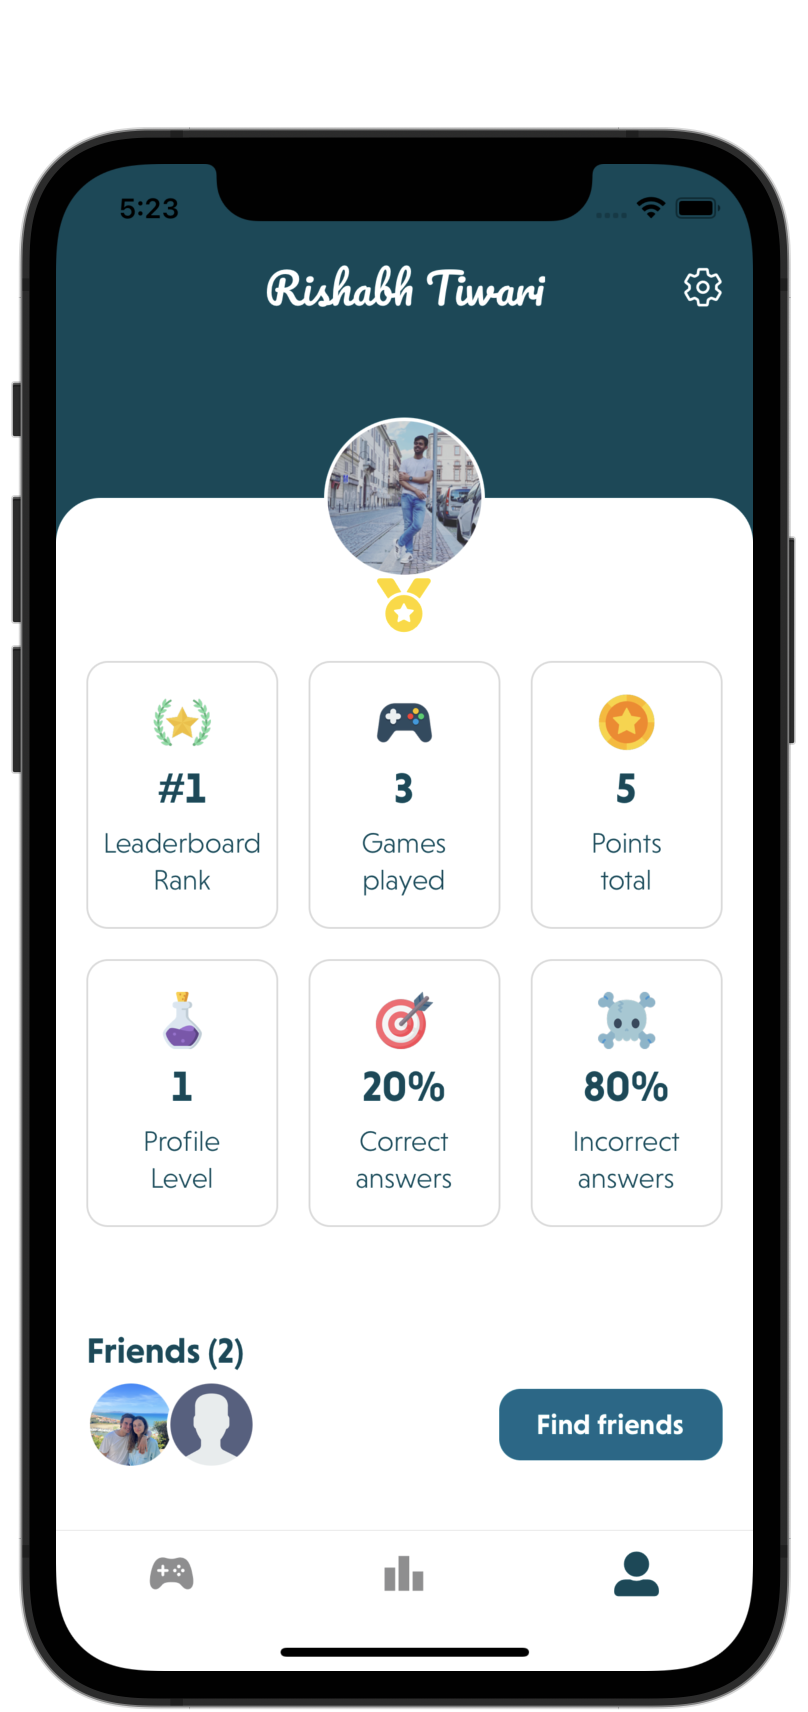
\includegraphics[width=\linewidth]{Screens_UI/My Profile.png}
        \caption{\textbf{User Profile UI with Statistics}}
    \end{minipage}
\end{figure}


The Profile Page offers a comprehensive overview of the user's achievements and statistics within the BrainMe application. At the top, users can see their profile picture and username, providing a personalized touch. Below this, various statistics and achievements are displayed, including:

\begin{itemize}
\item \textbf{Leaderboard Rank:} Shows the user's current rank on the leaderboard, motivating them to improve their performance.
\item \textbf{Games Played:} Displays the total number of games the user has participated in.
\item \textbf{Points Total:} Indicates the total points accumulated by the user.
\item \textbf{Profile Level:} Represents the user's profile level based on their activity and achievements.
\item \textbf{Correct Answers:} Shows the percentage of questions the user has answered correctly.
\item \textbf{Incorrect Answers:} Displays the percentage of questions the user has answered incorrectly.
\end{itemize}

Additionally, there is a "Find Friends" button that allows users to search for and connect with other users within the app, enhancing the social learning experience. The clean and intuitive design ensures that users can easily access and understand their statistics, fostering a sense of achievement and encouraging continuous engagement with the app.

\subsubsection{Friend list and checking other user's profile}

The Friend List and Checking Other User's Profile feature in BrainMe enhances the social interaction aspect of the application. It allows users to view the friends they already follow and view their progress and achievements.

\begin{itemize}
\item \textbf{Friend List:} The left screen (Figure 33) displays the user's friends list. Users can see their friends' names, profile pictures, and the points they have earned. A search bar at the top allows users to quickly find specific friends by name.
\item \textbf{Friend's User Profile:} The right screen (Figure 34) shows a friend's detailed profile when selected from the friends list. The profile includes the friend's leaderboard rank, games played, total points, profile level, correct answer percentage, and incorrect answer percentage. Additionally, users can send a message or unfollow the friend using the buttons provided.
\end{itemize}

This feature promotes a competitive and collaborative environment, motivating users to improve their performance by comparing their achievements with those of their friends.



\begin{figure}[H]
    \centering
    \begin{minipage}[b]{0.43\linewidth}
        \centering
        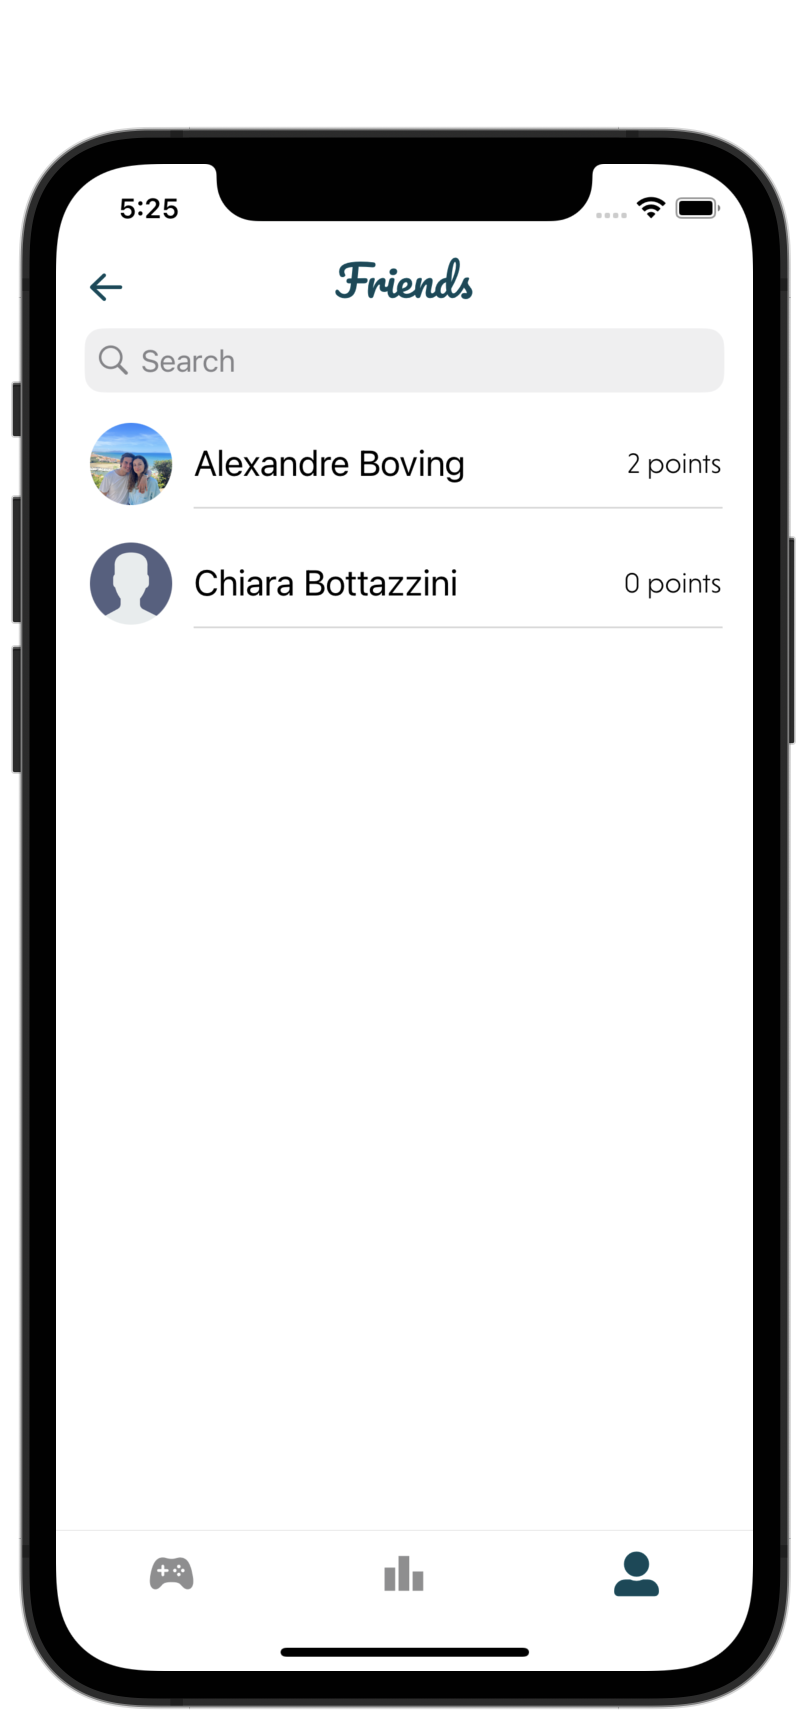
\includegraphics[width=\linewidth]{Mobile UI/Friend List.png}
        \caption{User's friends list}
    \end{minipage}
    \hspace{0.1\linewidth}
    \begin{minipage}[b]{0.43\linewidth}
        \centering
        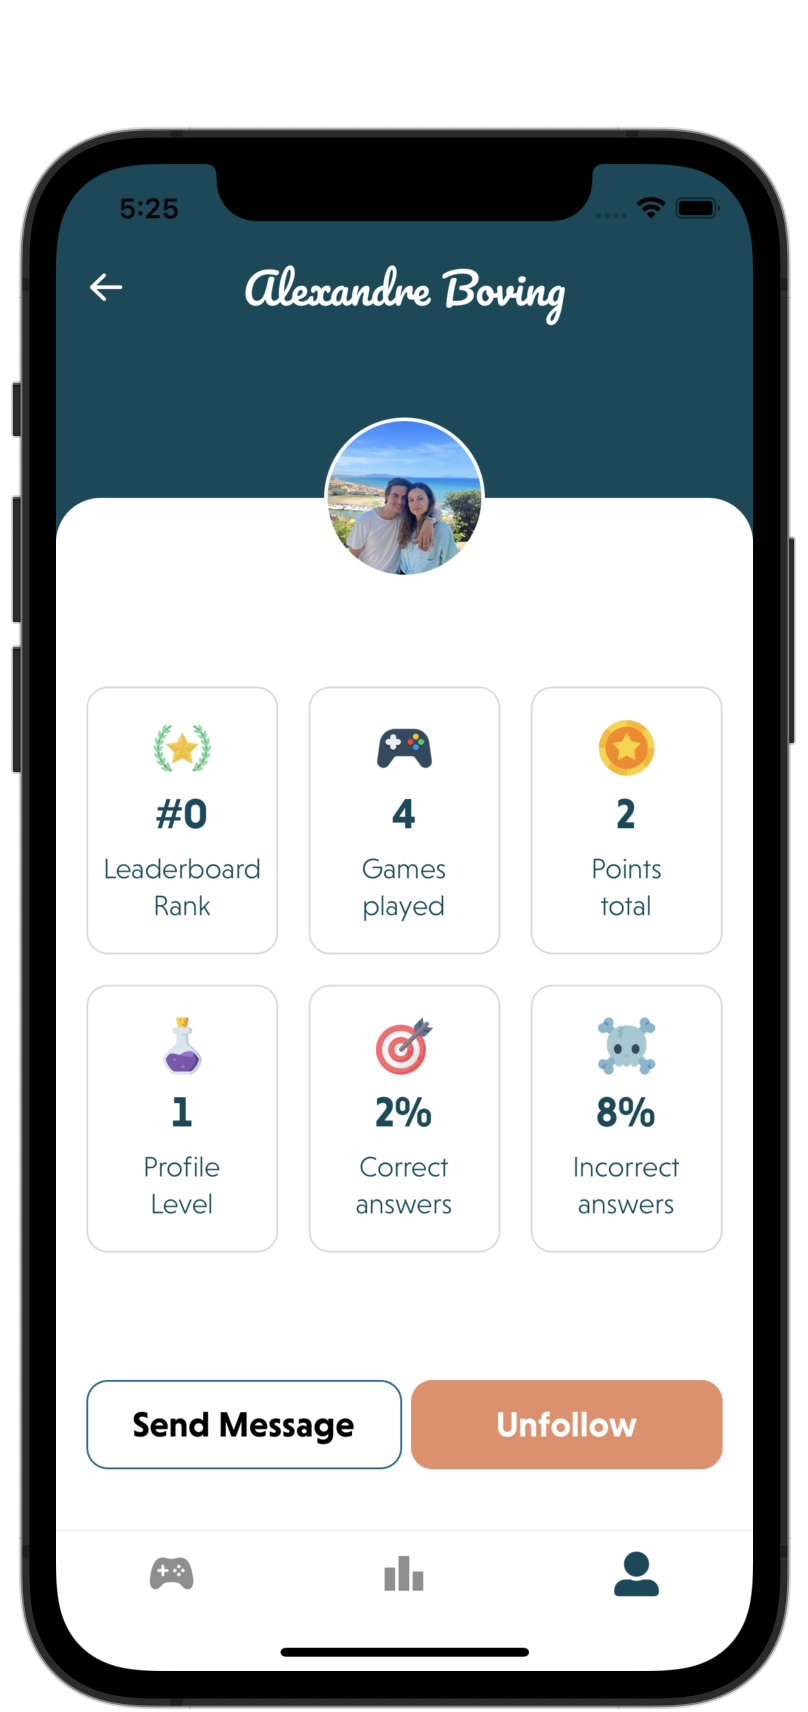
\includegraphics[width=\linewidth]{Mobile UI/Friend's Profile.png}
        \caption{Friend's User Profile}
    \end{minipage}
    \vspace{0.5cm}
    \caption{\textbf{User's friend list along with friend's user profile}}
\end{figure}

\subsubsection{Find Friends}

\begin{figure}[H]
    \centering
    \begin{minipage}[b]{0.43\linewidth}
        \centering
        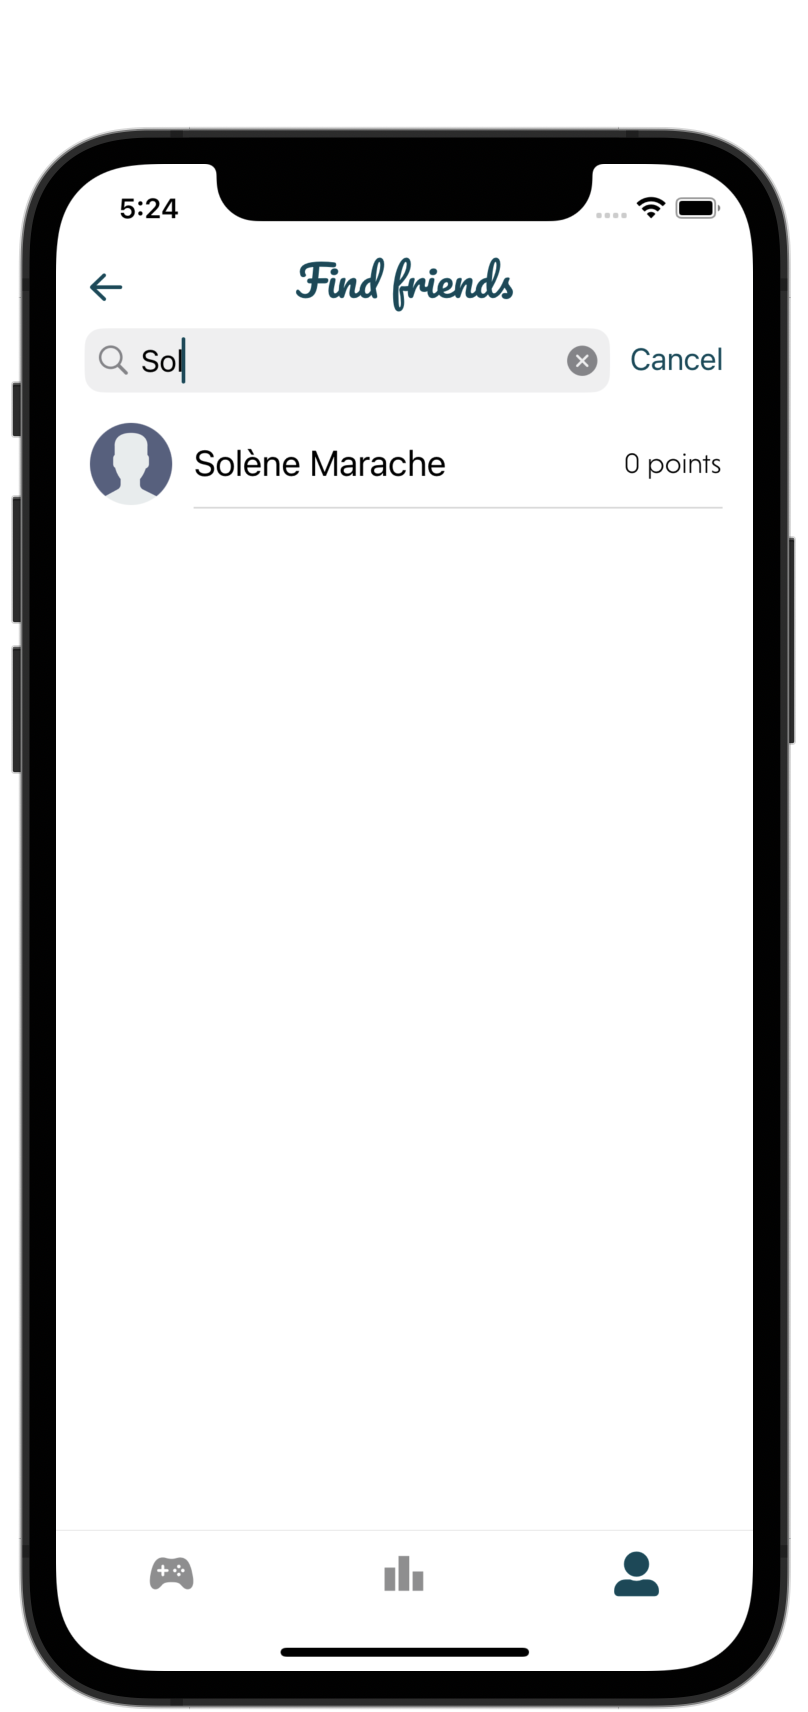
\includegraphics[width=\linewidth]{Mobile UI/Find Friends.png}
        \caption{Searching for a friend from the available users}
    \end{minipage}
    \hspace{0.1\linewidth}
    \begin{minipage}[b]{0.43\linewidth}
        \centering
        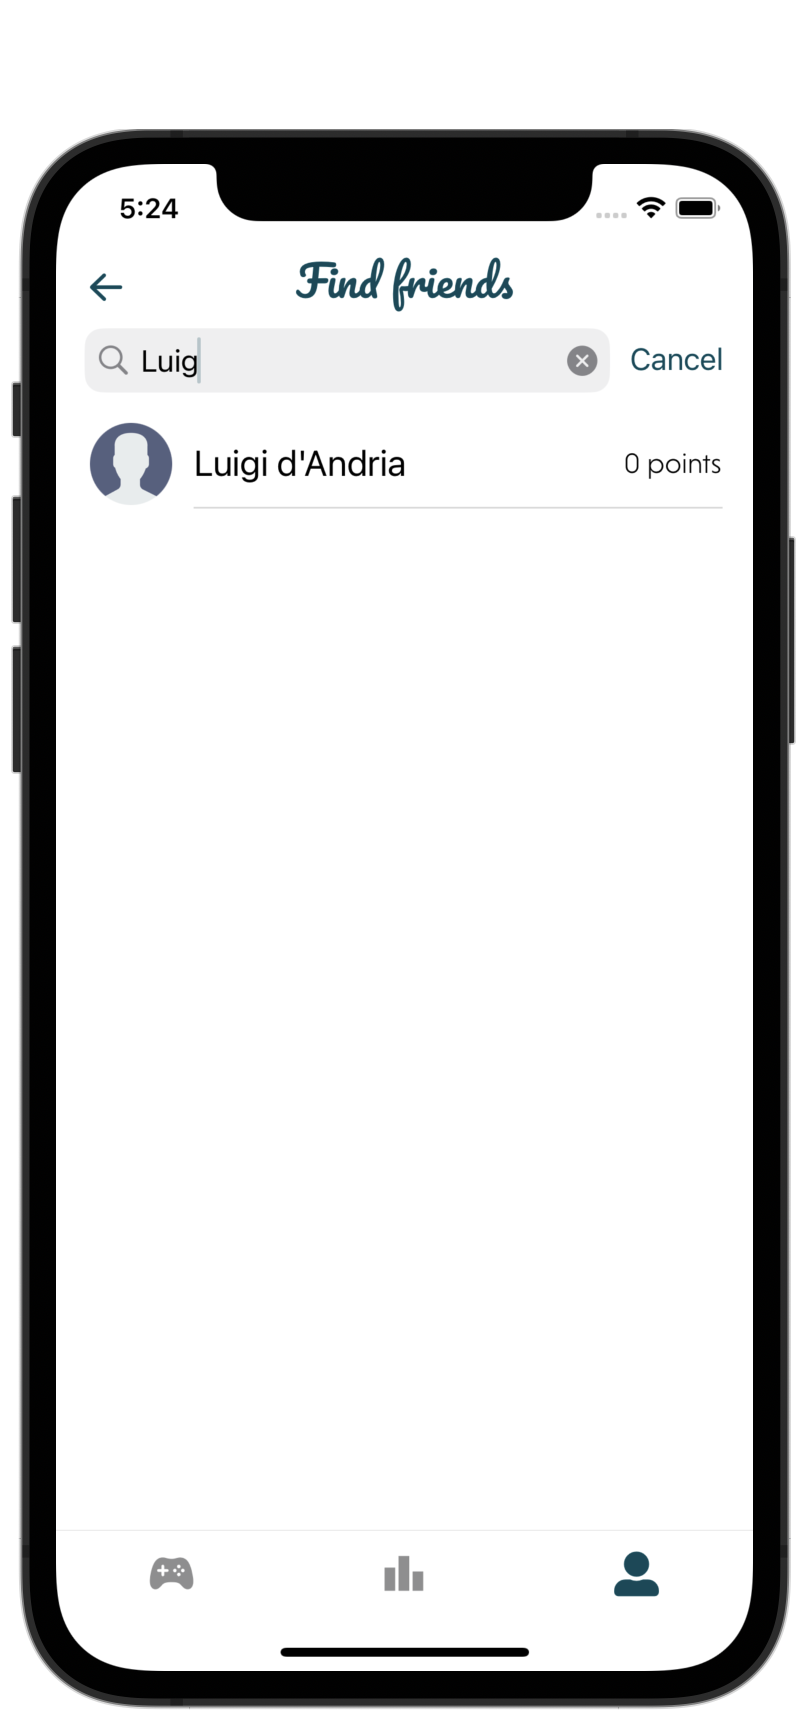
\includegraphics[width=\linewidth]{Mobile UI/Find Friends 1.png}
        \caption{Filter search for following a friend}
    \end{minipage}
    \vspace{0.5cm}
    \caption{\textbf{User can search for a friend and follow them}}
\end{figure}

The Find Friends feature in BrainMe allows users to search for and connect with other users. This promotes social interaction and collaboration within the application.

\begin{itemize}
\item \textbf{Searching for a Friend:} The left screen (Figure 36) shows the user entering a friend's name into the search bar. As the user types, the app filters the list to display matching names. This makes it easy for users to find specific friends quickly.
\item \textbf{Filter Search for Adding:} The right screen (Figure 37) displays the results of the search, showing the user’s profile picture, name, and points. Users can select a friend from the list to view their profile and follow them.
\end{itemize}

\subsubsection{Chat Page}

\begin{figure}[H]
    \centering
    \begin{minipage}[b]{0.43\linewidth}
        \centering
        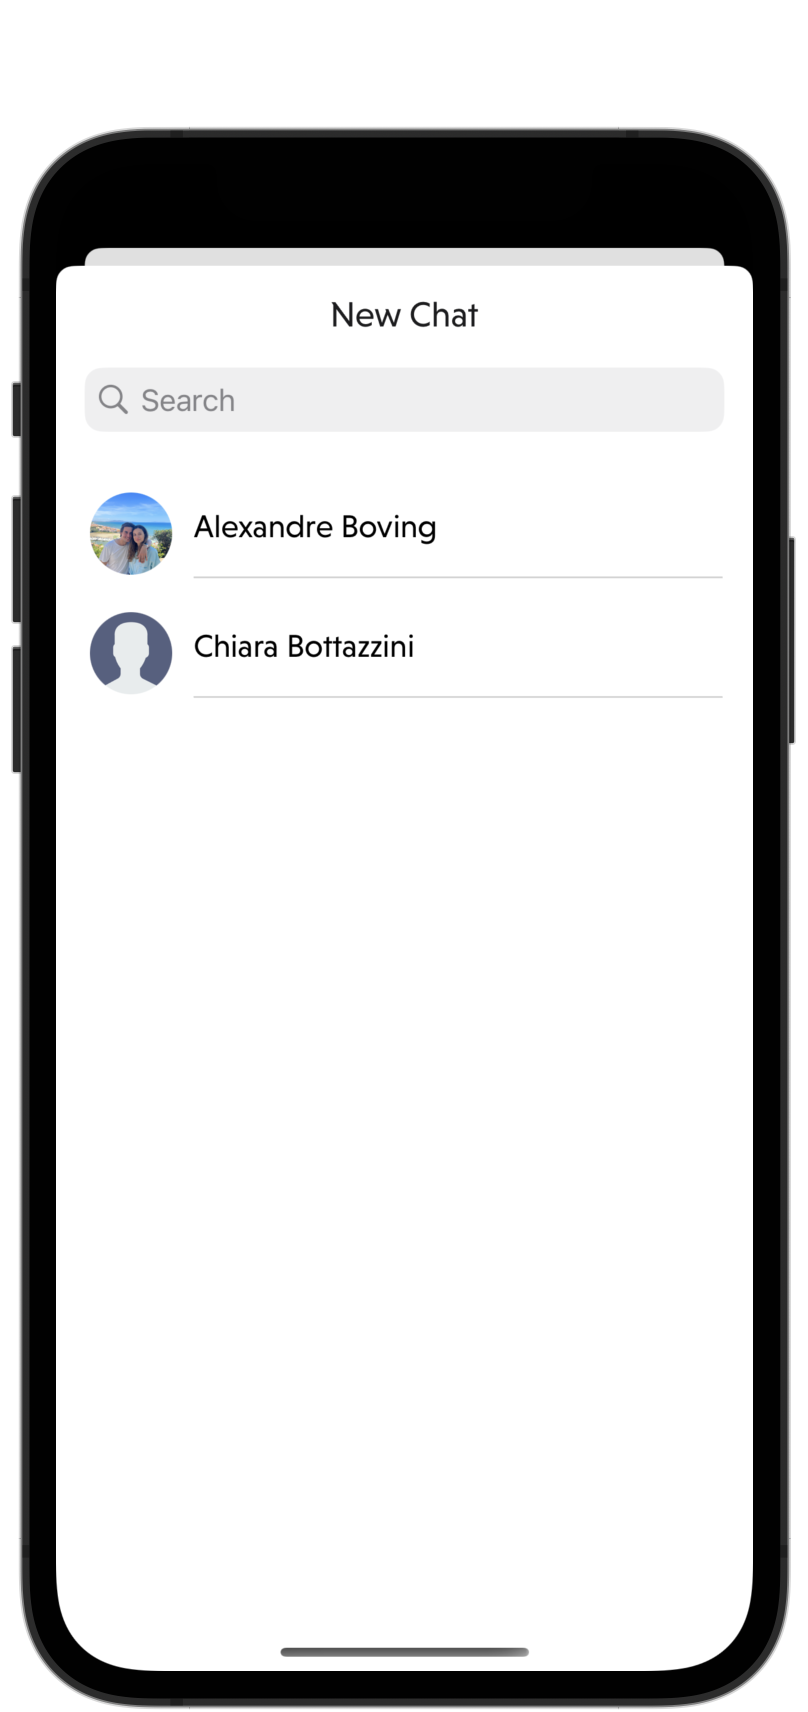
\includegraphics[width=\linewidth]{Images/New Chat Selection.png}
        \caption{Creating new chat}
    \end{minipage}
    \hspace{0.1\linewidth}
    \begin{minipage}[b]{0.43\linewidth}
        \centering
        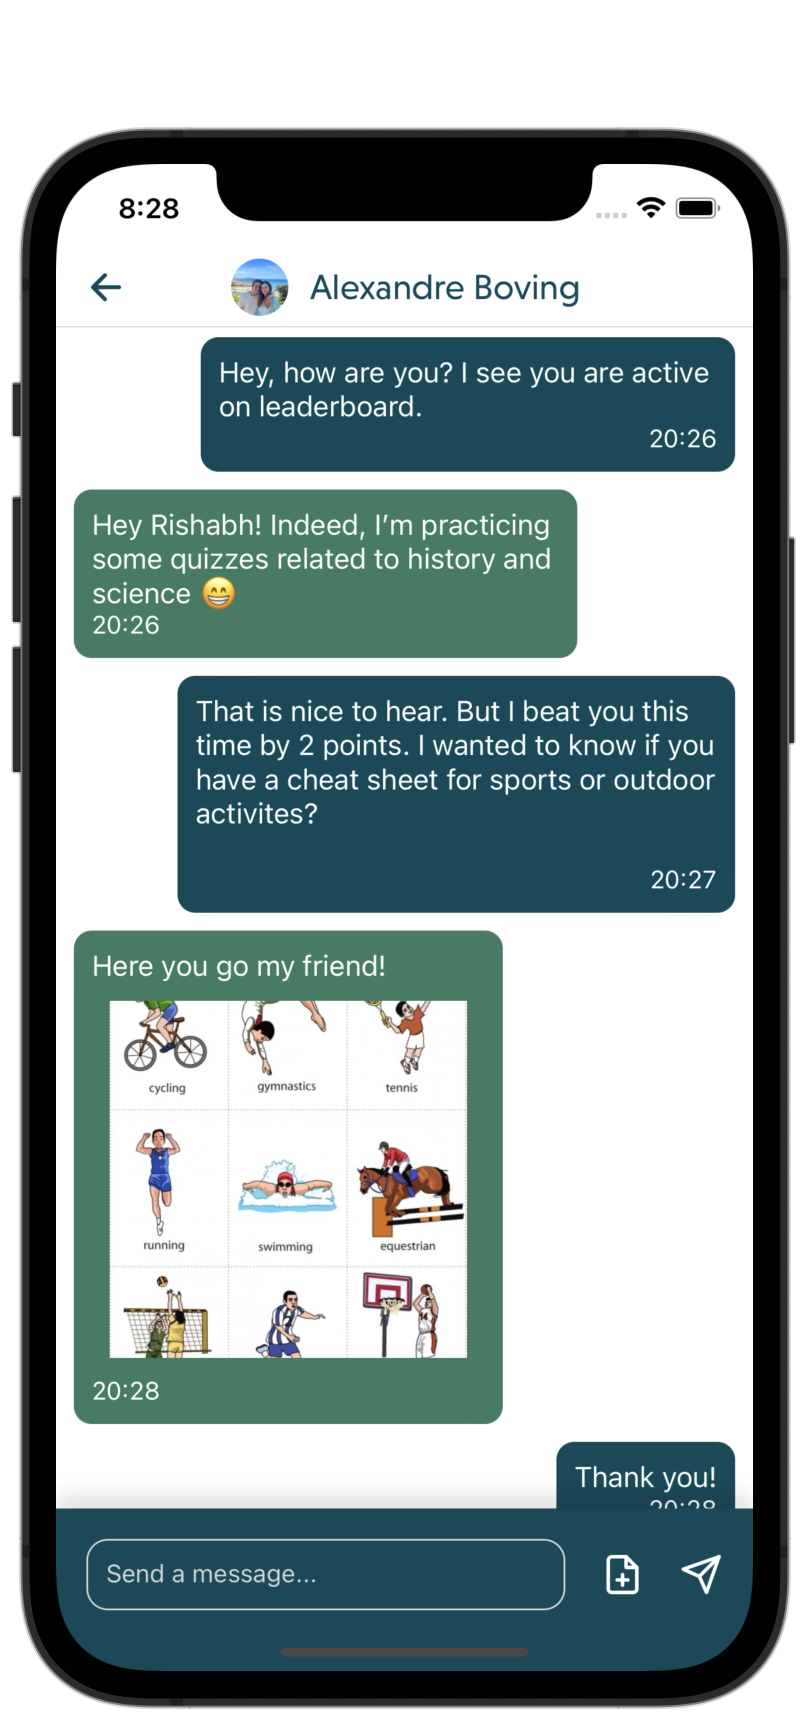
\includegraphics[width=\linewidth]{Images/Chat Example.png}
        \caption{Chat System Example}
    \end{minipage}
    \vspace{0.5cm}
    \caption{\textbf{Creation and an example of a new chat with file sharing}}
\end{figure}

The chat page allows users to create new chats and engage in conversations with other users. This feature supports both text and file sharing, enhancing the communication experience within the app.

\begin{itemize}
    \item \textbf{Creating New Chat:} Users can easily initiate a new chat with their friends by selecting from a list of contacts.
    \item \textbf{Chat System Example:} The chat interface displays messages exchanged between users, including the time stamps and any shared files.
    \item \textbf{File Sharing:} Users can share images and other files within the chat, making it more interactive and engaging.
\end{itemize}

\vspace{1cm}

\subsubsection{Settings Page}

The Settings Page in BrainMe provides users with the ability to manage their account details and preferences, ensuring a personalized and secure experience.

\begin{itemize}
\item \textbf{Account Settings Page:} The left screen (Figure 39) shows the account settings page where users can view and update their personal information, such as their name and family name. This screen also includes options for managing push notifications and account security, like signing out or deleting the account.
\item \textbf{Push Notifications:} The right screen (Figure 40) displays the toggle switch for push notifications. Users can easily turn notifications on or off according to their preference, ensuring they stay informed about important updates without being overwhelmed.
\end{itemize}

\begin{figure}[H]
    \centering
    \begin{minipage}[b]{0.43\linewidth}
        \centering
        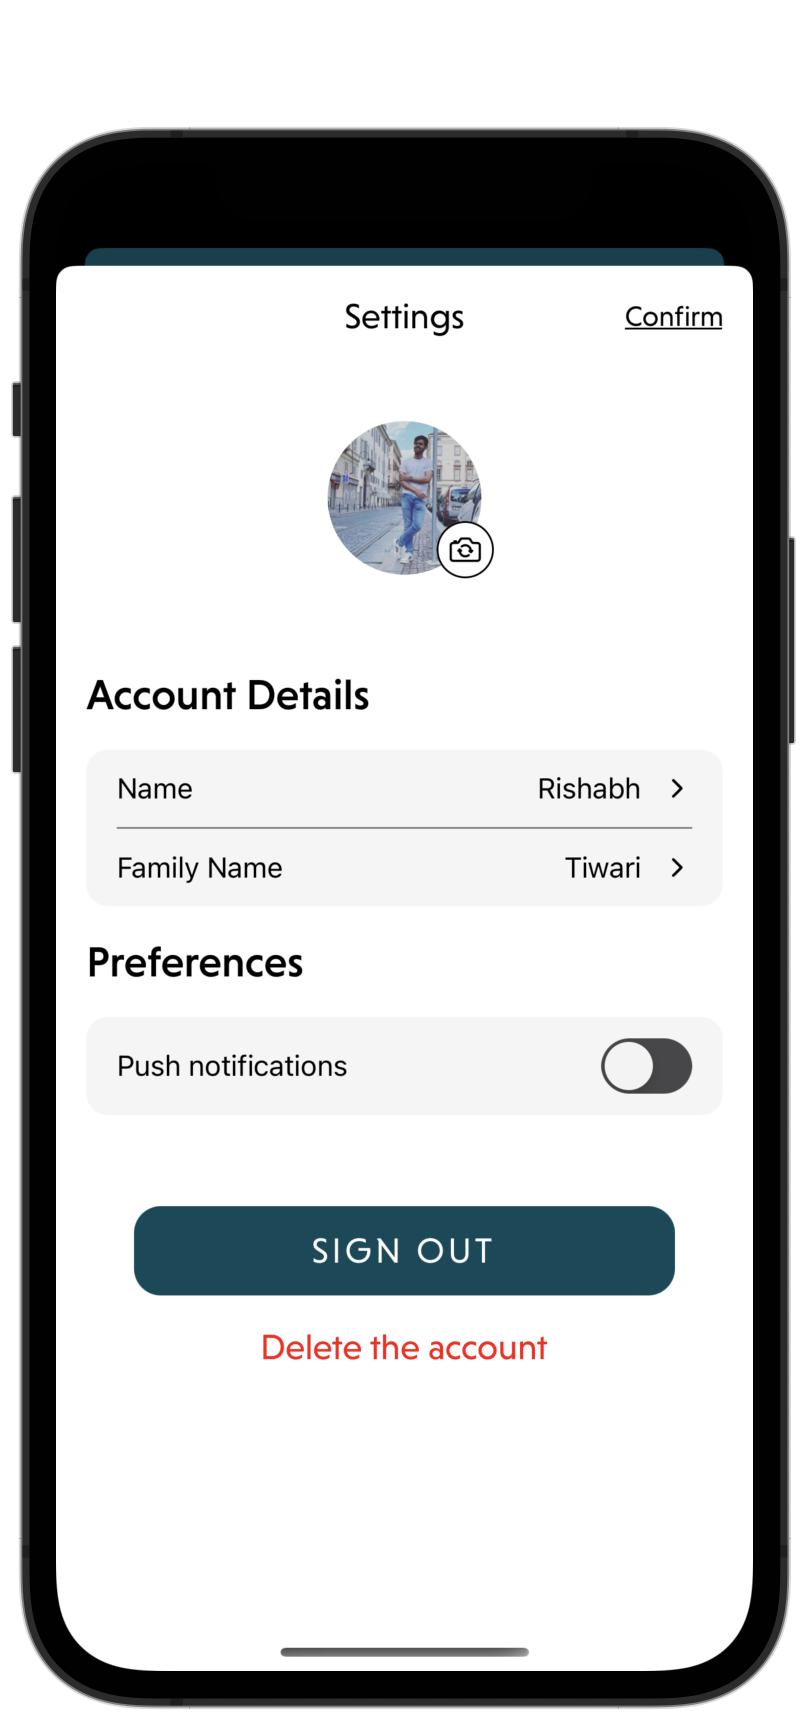
\includegraphics[width=\linewidth]{Mobile UI/Account Settings.png}
        \caption{Account Settings Page}
    \end{minipage}
    \hspace{0.1\linewidth}
    \begin{minipage}[b]{0.43\linewidth}
        \centering
        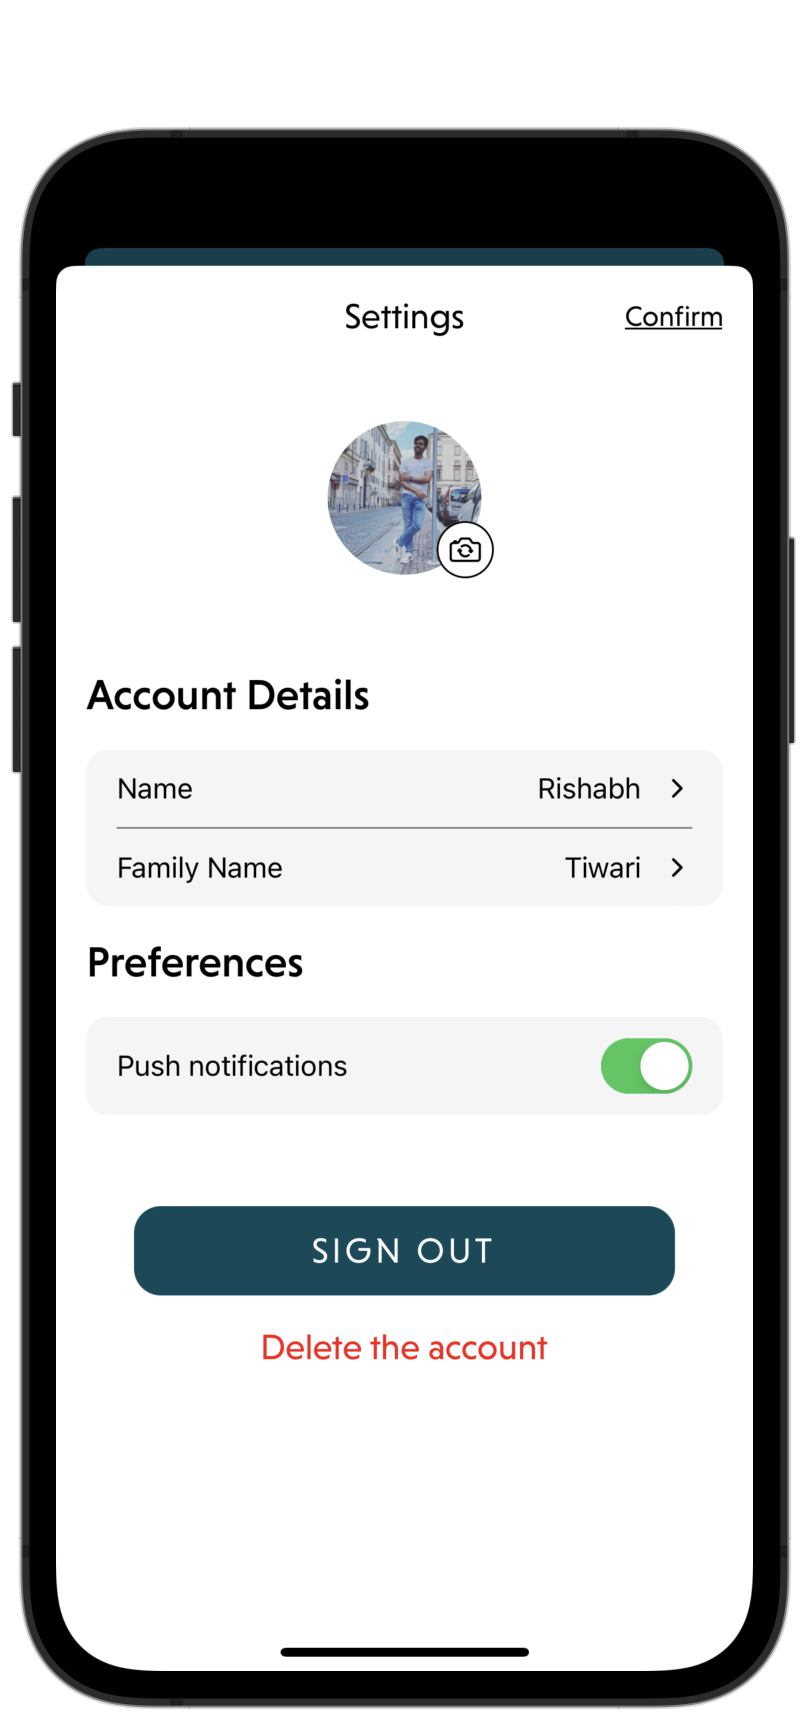
\includegraphics[width=\linewidth]{Mobile UI/Push Notifications.png}
        \caption{Push Notifications}
    \end{minipage}
    \vspace{0.5cm}
    \caption{\textbf{Account Settings with Push Notifications}}
\end{figure}



\subsection{Tablet UI}
\subsubsection{Login Page and SignUp Page}


\begin{figure}[H]
    \centering
    \begin{minipage}[b]{0.43\linewidth}
        \centering
        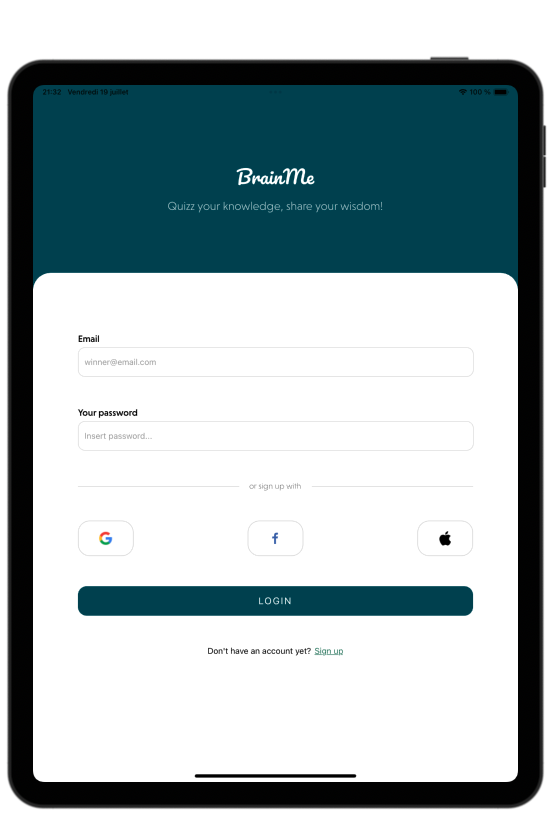
\includegraphics[height=10cm]{TabletUI/Login Page.png}
        \caption{Login Page}
    \end{minipage}
    \hspace{0.1\linewidth}
    \begin{minipage}[b]{0.43\linewidth}
        \centering
        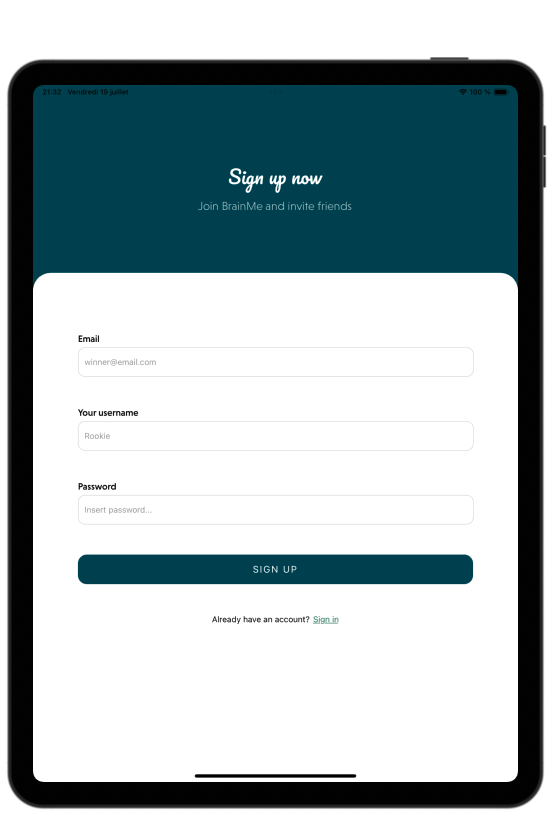
\includegraphics[height=10cm]{TabletUI/Sign Up Page.png}
        \caption{Sign Up Page}
    \end{minipage}
    \vspace{0.5cm}
    \caption{\textbf{The BrainMe Application}}
\end{figure}

The above screen performs the same functions as the Ipphone screens. The user can sign up and login using the respective email or single sign on methods.

\subsubsection{Quiz Page: }

\begin{figure}[H]
    \centering
    \begin{minipage}[b]{0.43\linewidth}
        \centering
        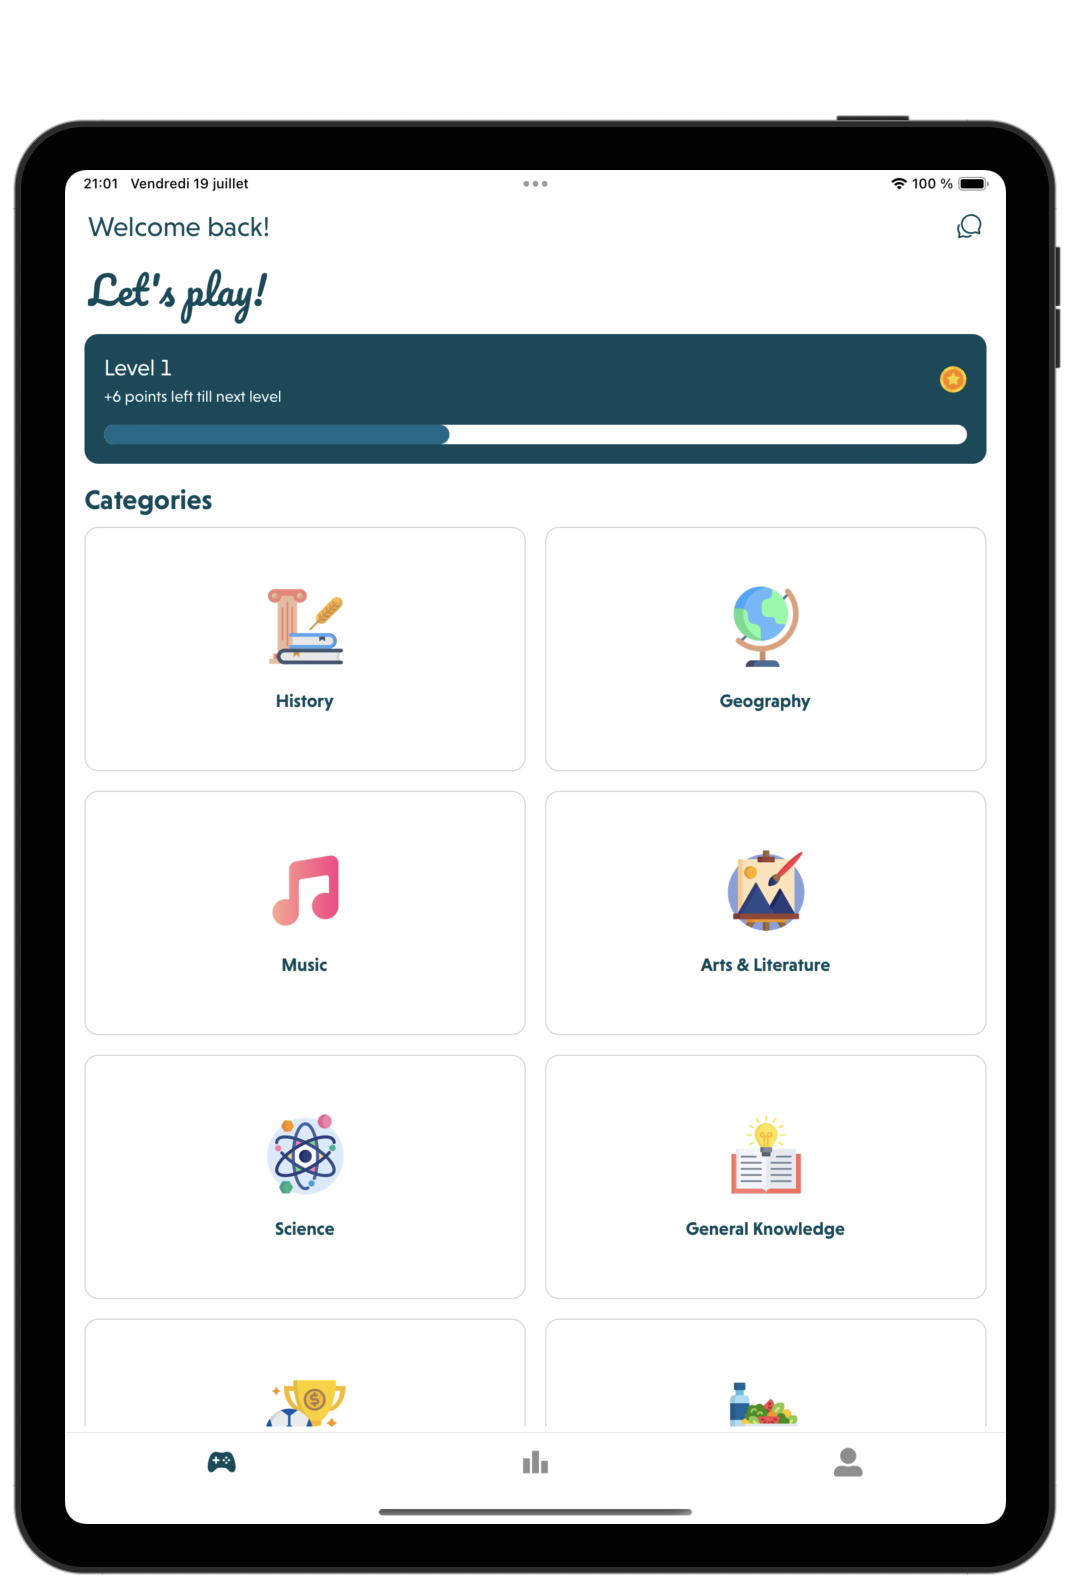
\includegraphics[height=10cm]{TabletUI/Quiz Page 1.png}
        \caption{Quiz Page 1}
    \end{minipage}
    \hspace{0.1\linewidth}
    \begin{minipage}[b]{0.43\linewidth}
        \centering
        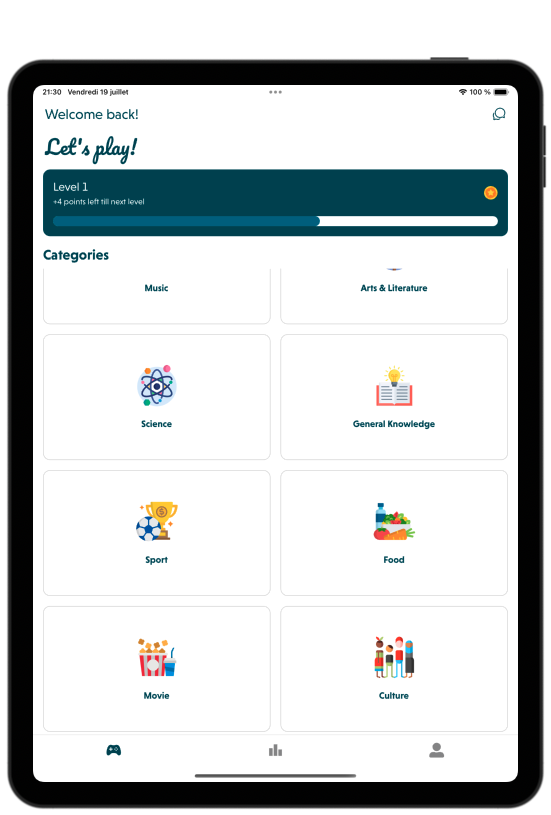
\includegraphics[height=10cm]{TabletUI/Quiz Page 2.png}
        \caption{Quiz Page 2}
    \end{minipage}
    \vspace{0.5cm}
    \caption{\textbf{The BrainMe Application All Quiz Categories}}
\end{figure}

The Ipad screen allows the user to have a more wider and bigger aspects of the icons and the text which is the major difference between the Iphone and the Ipad. The user here can select from various categories to begin the quiz.

\subsubsection{Quiz Levels}

\begin{figure}[H]
    \centering
    \begin{minipage}[b]{0.43\linewidth}
        \centering
        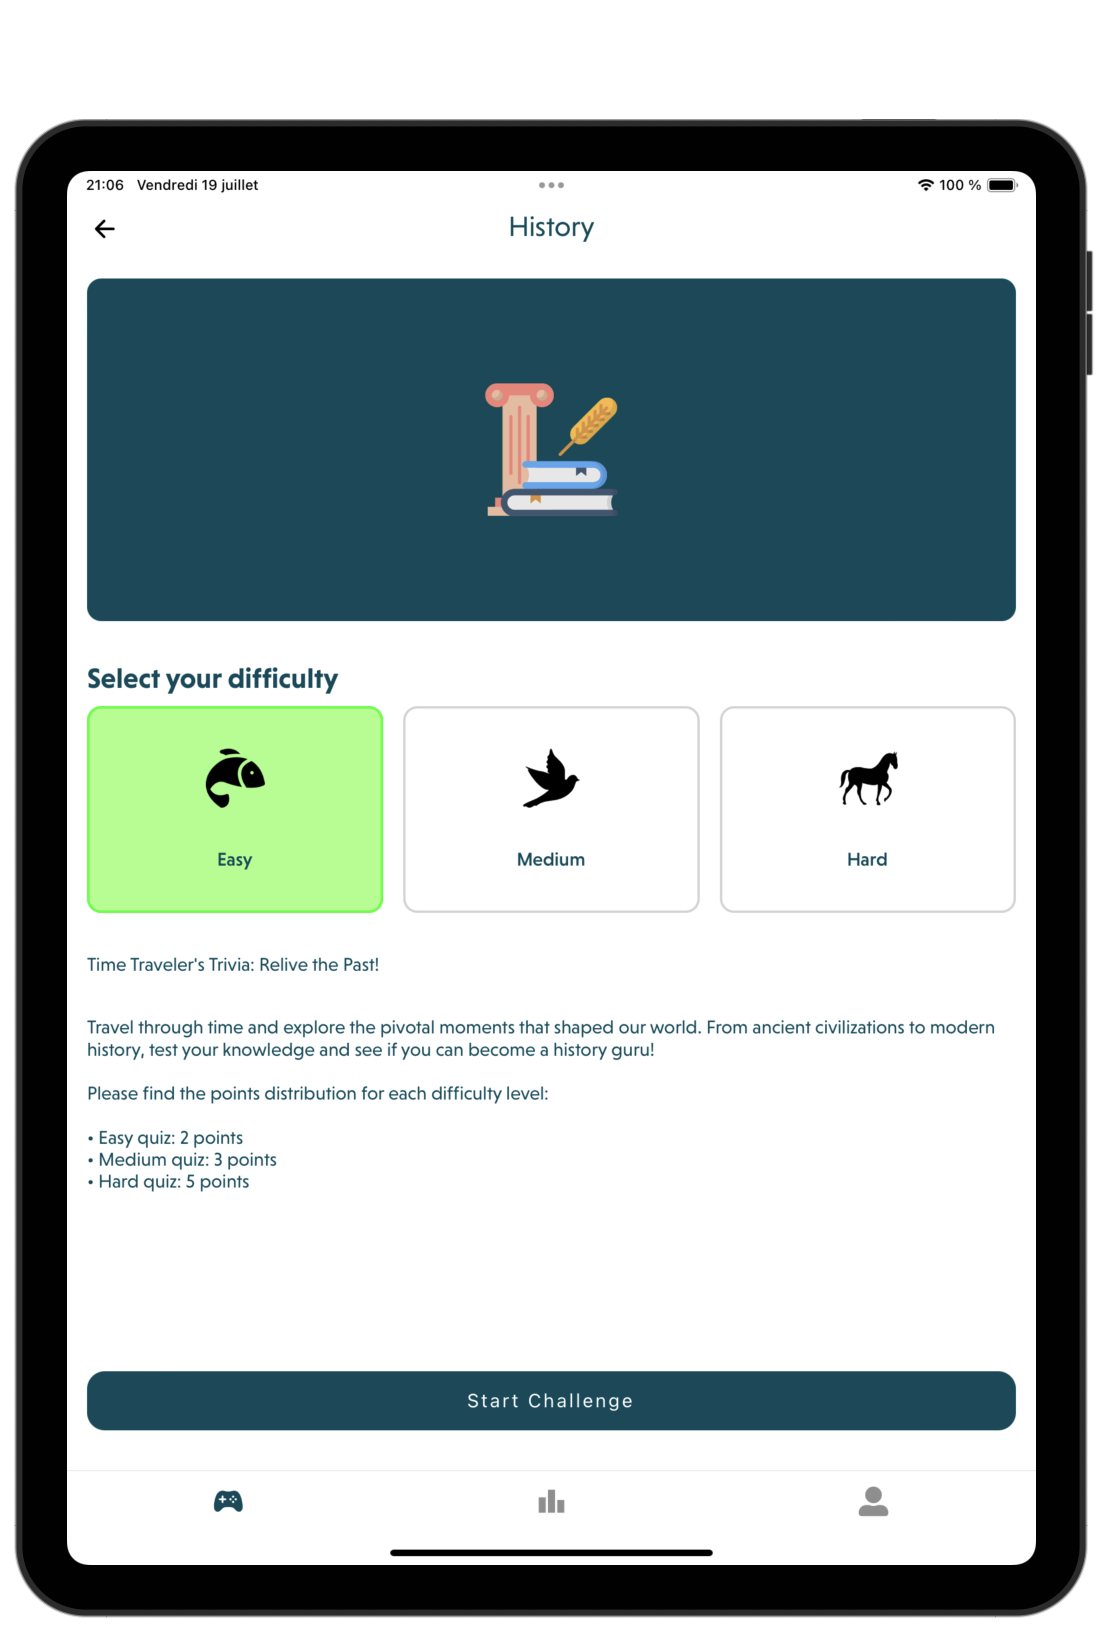
\includegraphics[height=10cm]{TabletUI/Easy Level Quiz.png}
        \caption{Easy Level Quiz}
    \end{minipage}
    \hspace{0.1\linewidth}
    \begin{minipage}[b]{0.43\linewidth}
        \centering
        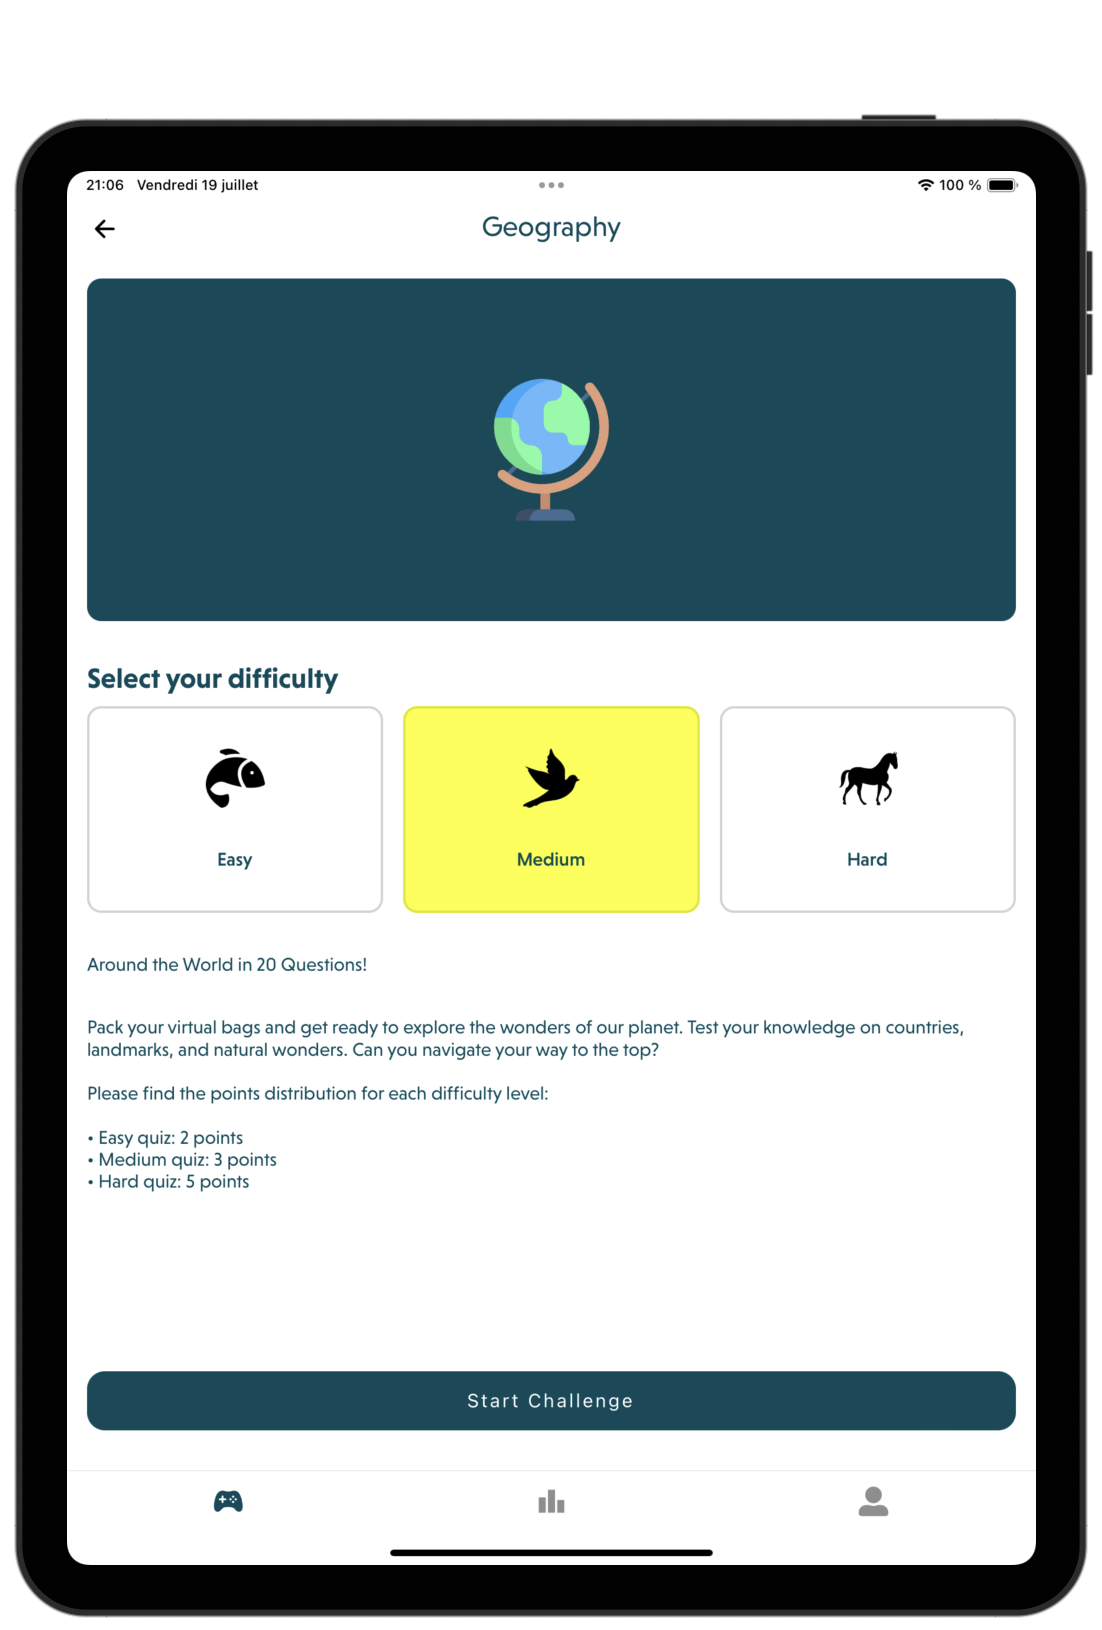
\includegraphics[height=10cm]{TabletUI/Medium Level Quiz.png}
        \caption{Medium Level Quiz}
    \end{minipage}
    \vspace{0.5cm}
    \caption{\textbf{Quiz Difficulty Description}}
\end{figure}

The above screen depicts the difficulty level the user can select from of different genres. THe user can select from easy medium and hard levels for the respective quiz and it will be more fun on Ipad or bigger screens to play or participate in the challenges.

\begin{figure}[H]
    \centering
    \begin{minipage}[b]{0.43\linewidth}
        \centering
        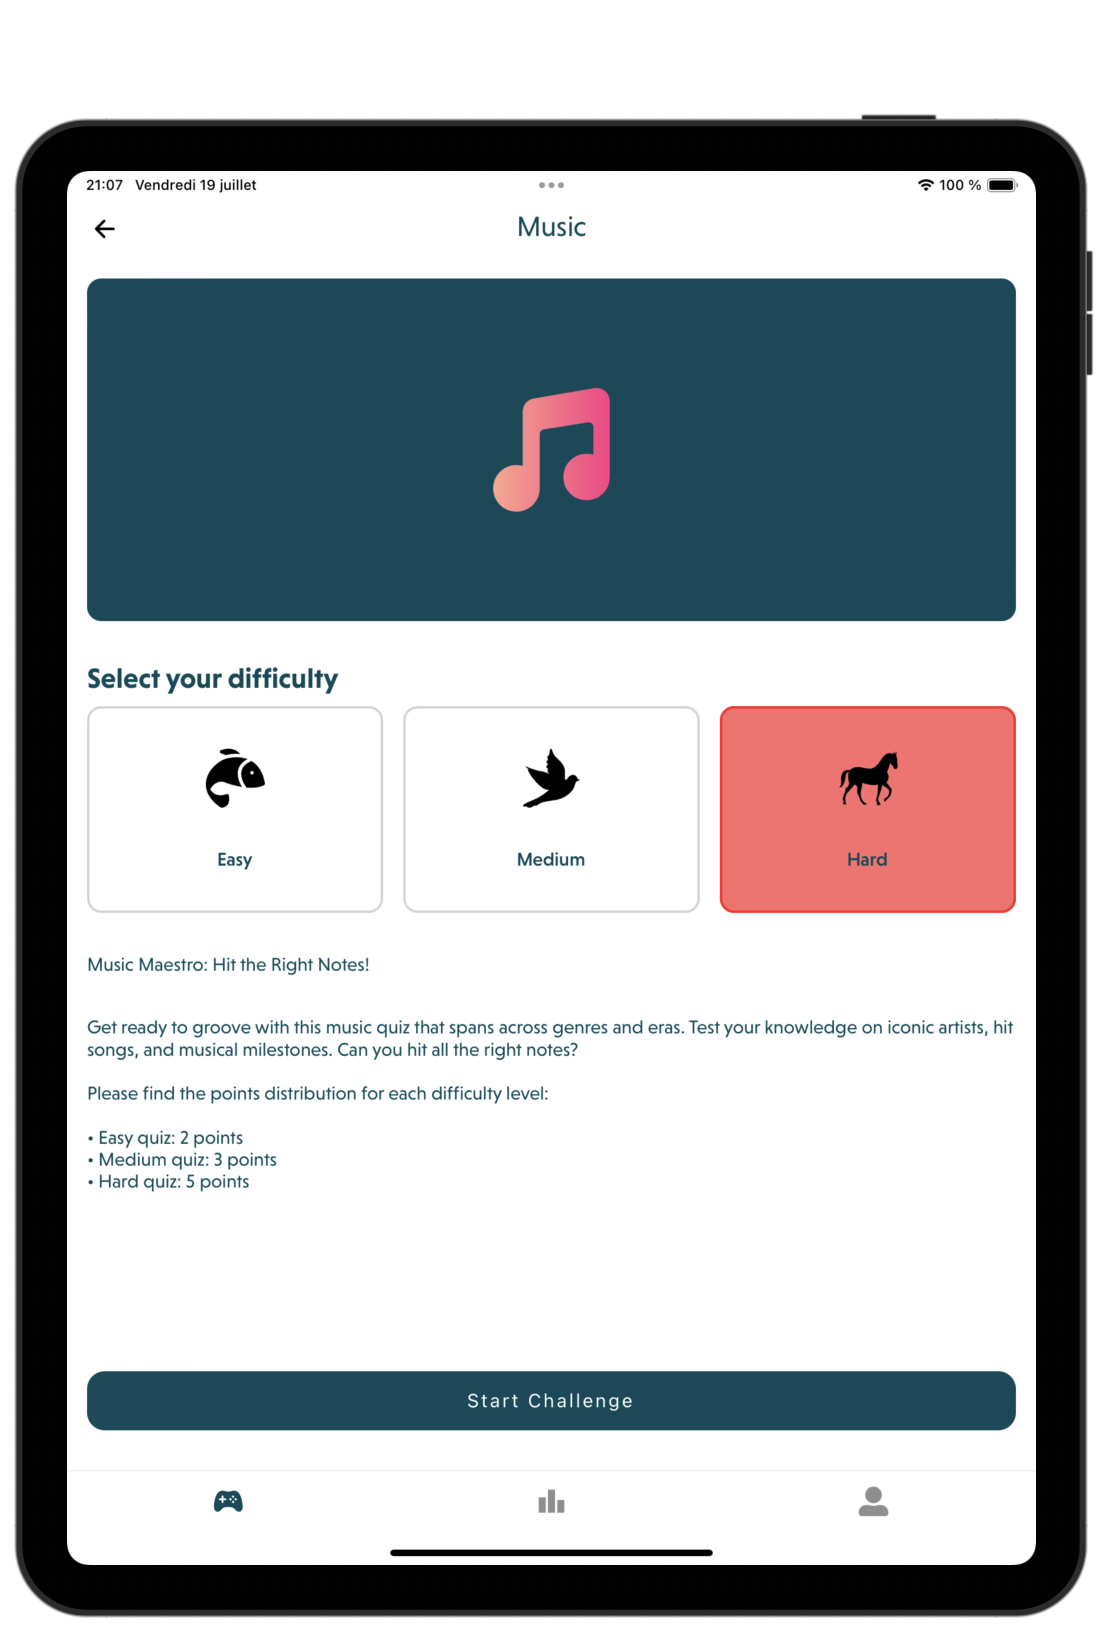
\includegraphics[height=10cm]{TabletUI/Hard Level Quiz.png}
        \caption{Hard Level Quiz}
    \end{minipage}
    \hspace{0.1\linewidth}
    \begin{minipage}[b]{0.43\linewidth}
        \centering
        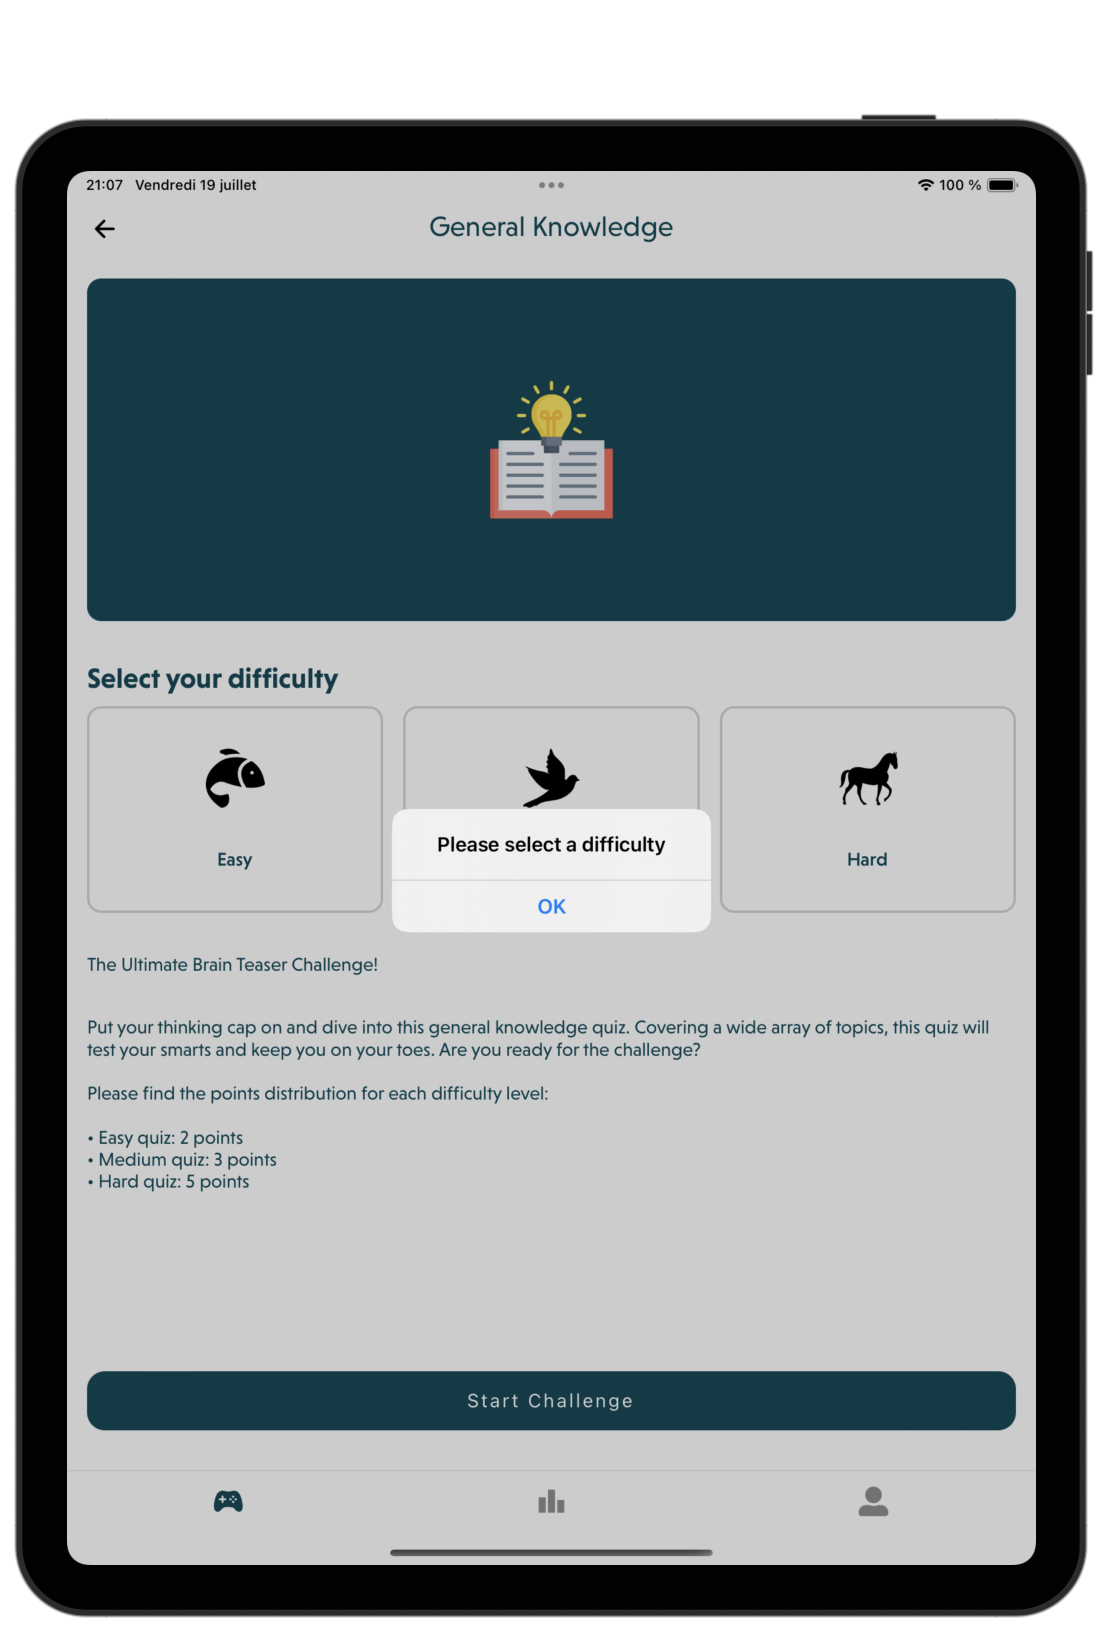
\includegraphics[height=10cm]{TabletUI/Select Difficulty.png}
        \caption{Select Difficulty}
    \end{minipage}
    \vspace{0.5cm}
    \caption{\textbf{Quiz Difficulty Description}}
\end{figure}

The user has to select a difficulty level in order to proceed. If the user does not make any selection, a alert box appears requesting the user to make a choice in order to proceed thus allowing more user engagement and making the application intuitive.

\subsubsection{Starting Quiz}

\begin{figure}[H]
    \centering
    \begin{minipage}[b]{0.43\linewidth}
        \centering
        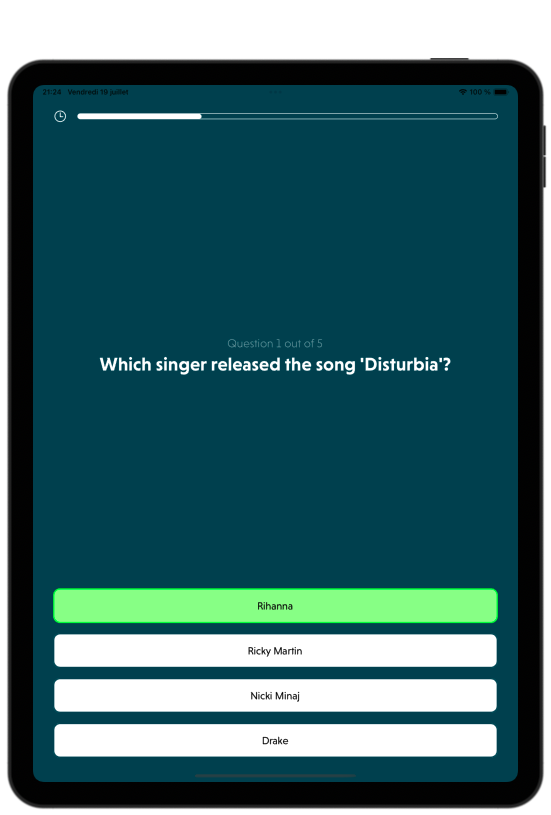
\includegraphics[height=10cm]{TabletUI/User selecting an option after starting a quiz.png}
        \caption{User selecting an option after starting a quiz}
    \end{minipage}
    \hspace{0.1\linewidth}
    \begin{minipage}[b]{0.43\linewidth}
        \centering
        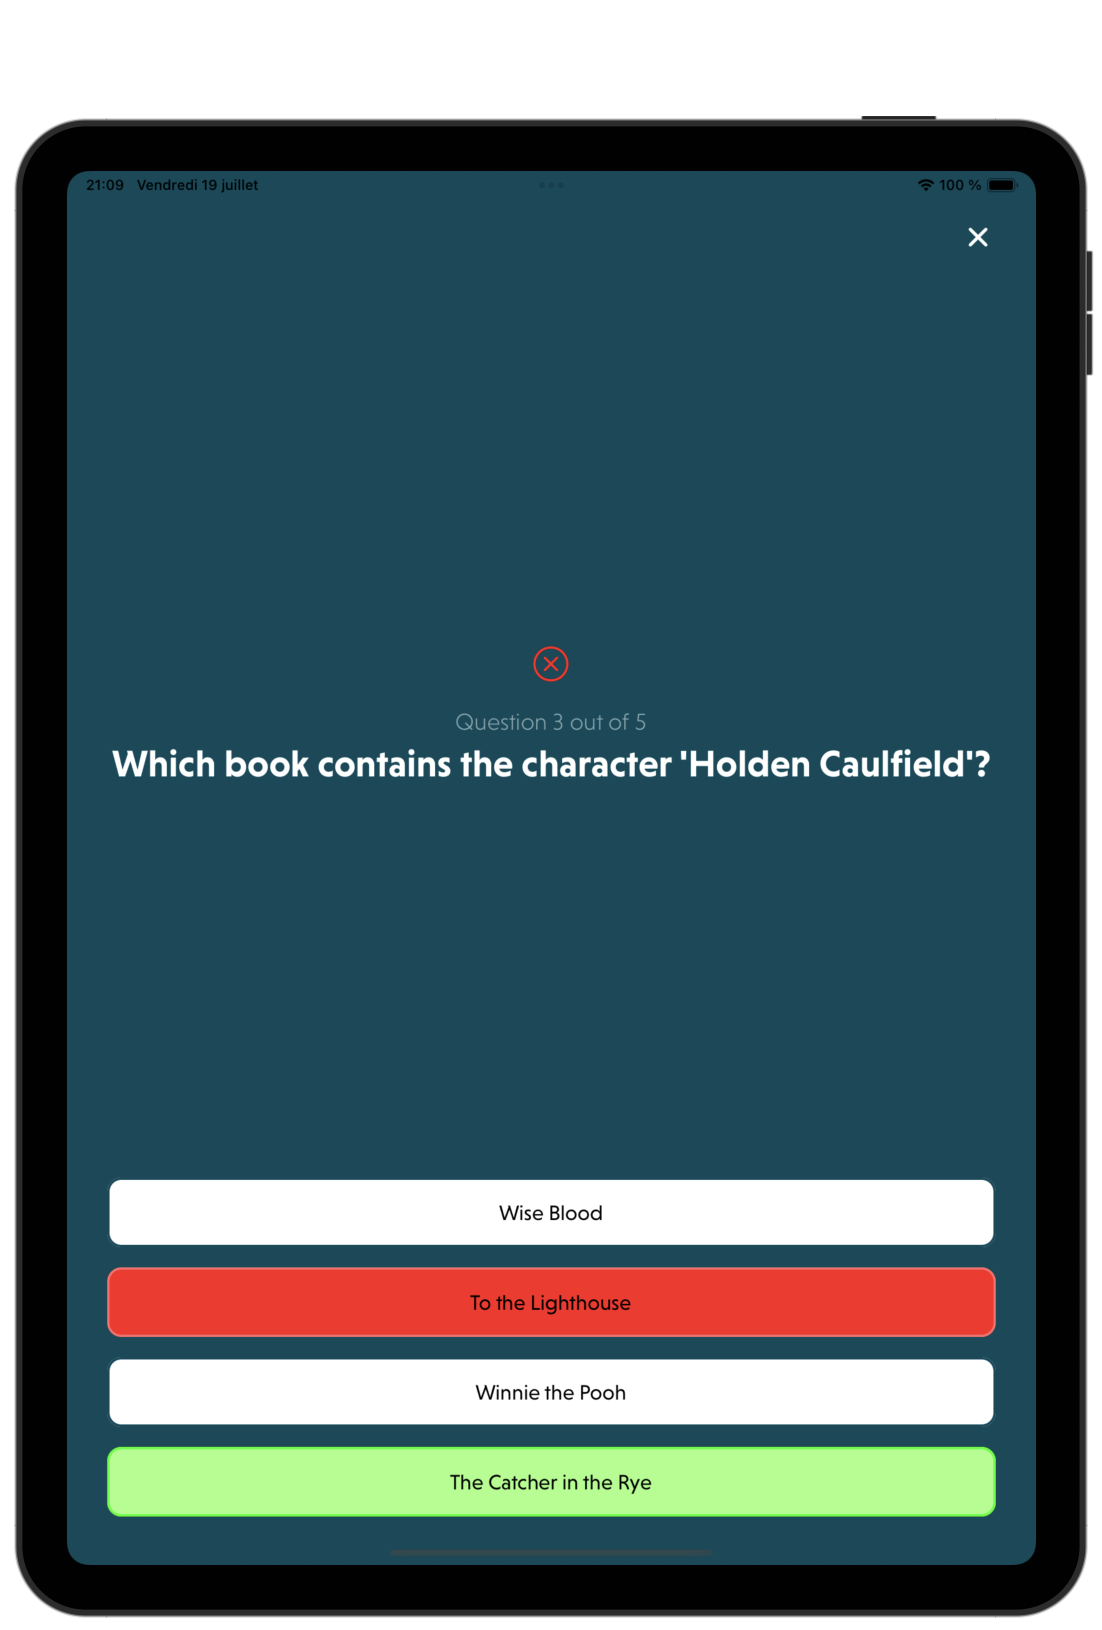
\includegraphics[height=10cm]{TabletUI/Showing the result after the time has ended.png}
        \caption{Showing the result after the time has ended}
    \end{minipage}
    \vspace{0.5cm}
    \caption{\textbf{Starting a quiz and selecting an option}}
\end{figure}

In this part of our application, just like the Iphone version, the user can start a quiz where the user gets 5 questions with a timer of 15 seconds and 4 options to select from based on the genre he has selected. Once the timer runs out, the user sees the solution if the choice made was correct or incorrect.

\subsubsection{Ending and Reviewing Quiz}

The ending and reviewing quiz screens provide users with a summary of their performance and an option to review their answers. These screens are designed to help users understand their mistakes and learn from them, enhancing the overall learning experience.

\begin{figure}[H]
    \centering
    \begin{minipage}[b]{0.43\linewidth}
        \centering
        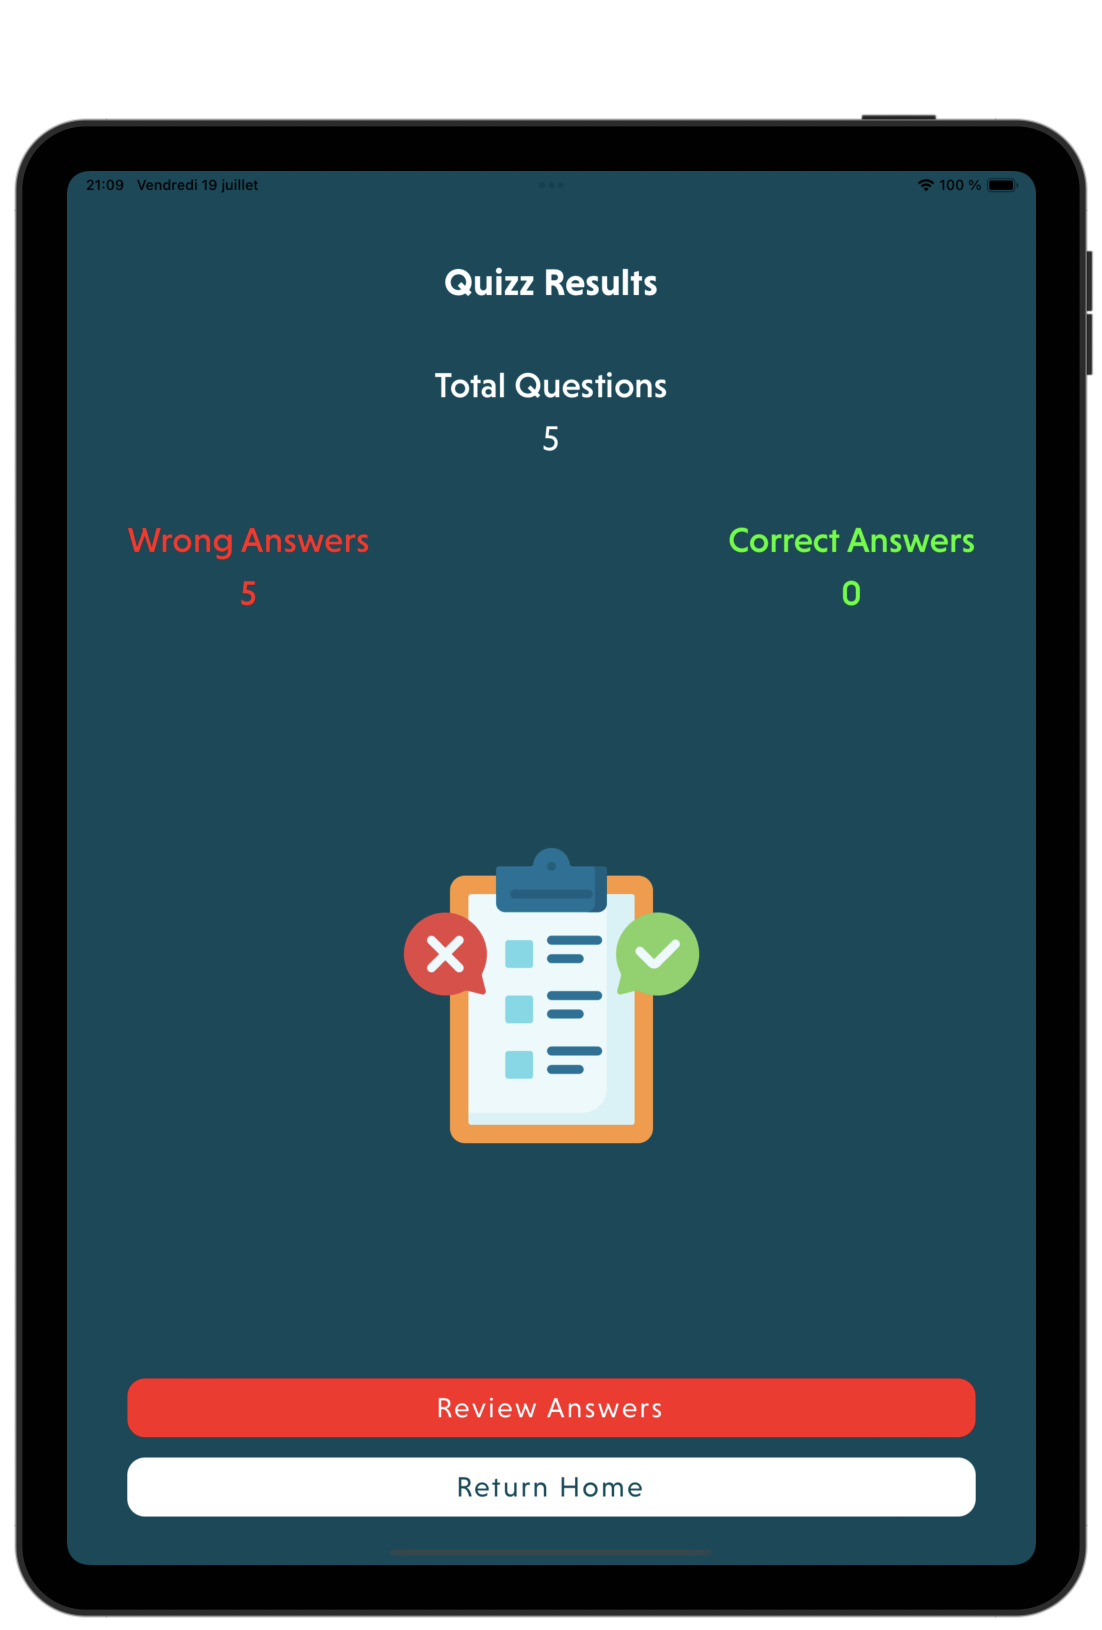
\includegraphics[width=\linewidth]{TabletUI/Quiz Results with options to review or return home.png}
        \caption{Quiz Results with options to review or return home}
    \end{minipage}
    \hspace{0.1\linewidth}
    \begin{minipage}[b]{0.43\linewidth}
        \centering
        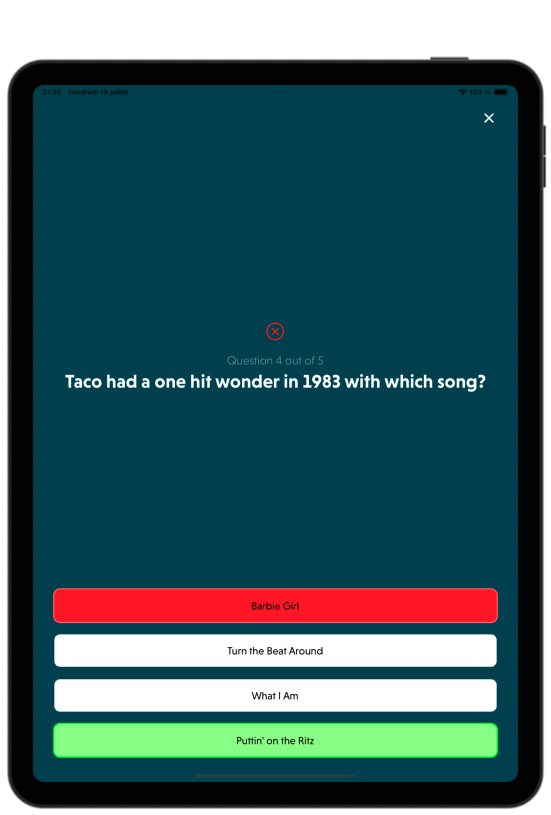
\includegraphics[width=\linewidth]{TabletUI/Displaying correct result for incorrect solution.png}
        \caption{Displaying correct result for incorrect solution}
    \end{minipage}
    \vspace{0.5cm}
    \caption{\textbf{Ending a quiz and selecting an option}}
\end{figure}

The user has the option to review their answers by tapping the "Review Answers" button.
If the user chooses to review their answers:
    \begin{itemize}
        \item The quiz review screen displays each question along with the user's selected answer and the correct answer.
        \item Correct answers are highlighted in green icon, while incorrect answers are highlighted in red icon.
    \end{itemize}
The user can also choose to return to the home page by tapping the "Return Home" button. \\\\
The below images share a glimpse of how the user can review it. If the user has selected the correct option, a green tick appears on the top and if the user has made no selection, then a red cross appears on the top and the correct solution is displayed.

\begin{figure}[H]
    \centering
    \begin{minipage}[b]{0.43\linewidth}
        \centering
        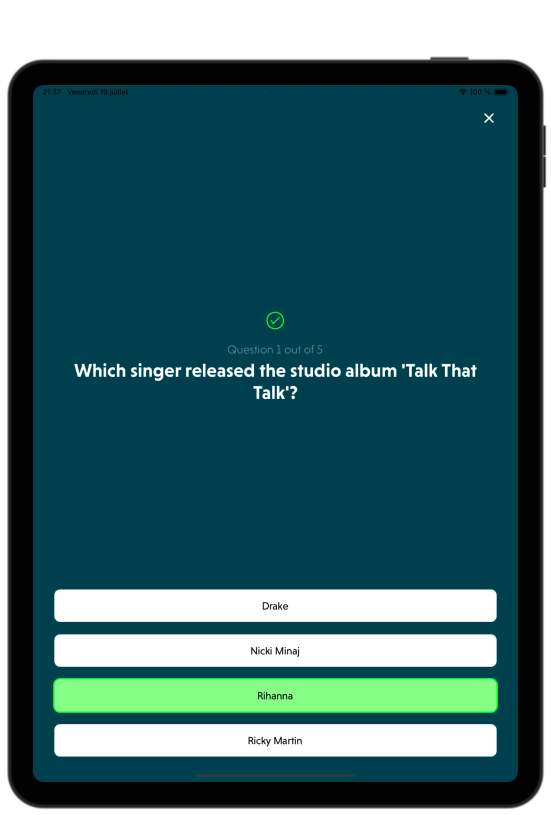
\includegraphics[width=\linewidth]{TabletUI/Reviewing correct solution for correct solution.png}
        \caption{Reviewing correct solution for correct selection}
    \end{minipage}
    \hspace{0.1\linewidth}
    \begin{minipage}[b]{0.43\linewidth}
        \centering
        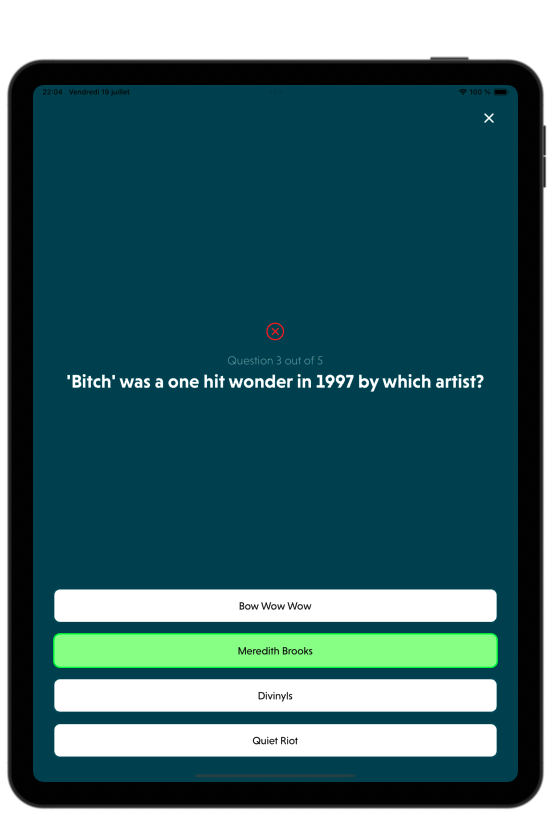
\includegraphics[width=\linewidth]{TabletUI/Reviewing correct solution for no selection.png}
        \caption{Reviewing correct solution for no selection}
    \end{minipage}
    \vspace{0.5cm}
    \caption{\textbf{Reviewing the correct result}}
\end{figure}


\vspace{1cm}

\subsubsection{Leaderboard}

The leaderboard feature in the BrainMe application displays the ranking of users based on their quiz performance. This promotes a competitive environment, motivating users to improve their scores and climb the ranks. Users can view their position relative to others, fostering a sense of achievement and encouraging active participation in quizzes.

\begin{figure}[H]
    \centering
    \begin{minipage}[b]{0.43\linewidth}
        \centering
        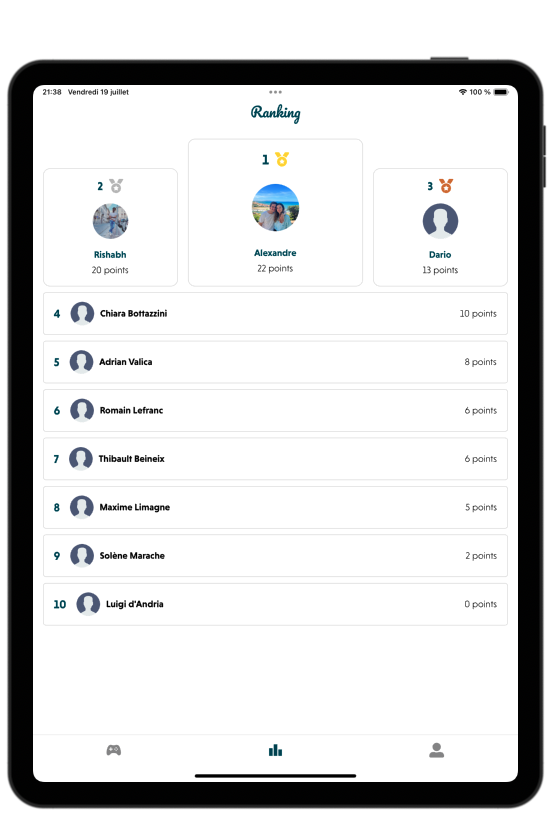
\includegraphics[width=\linewidth]{TabletUI/Leaderboard ranking depicting medals and rankings.png}
        \caption{Leaderboard ranking depicting medals and rankings}
    \end{minipage}
    \hspace{0.02\linewidth}
    \begin{minipage}[b]{0.43\linewidth}
        \centering
        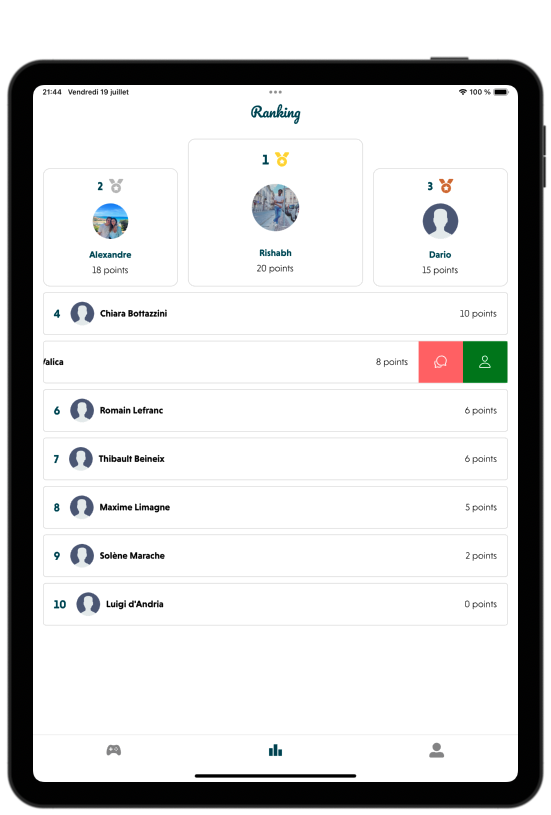
\includegraphics[width=\linewidth]{TabletUI/Sliding on the name to chat or view profile.png}
        \caption{Sliding on the name to chat or view profile}
    \end{minipage}
    \caption{\textbf{Leaderboard ranking and the medals along with chat option}}
\end{figure}


\begin{itemize}
\item \textbf{Real-time updates:} The leaderboard is updated in real-time to reflect the latest user rankings based on quiz performance.
\item \textbf{Visual indicators:} Medals for the top three users provide immediate visual recognition of the leading participants.
\item \textbf{User details:} Displaying usernames and profile pictures makes the leaderboard more personal and engaging.
\item \textbf{Sliding feature} Allows registered users to send message or view their profile directly from the leaderboard rankings.
\item \textbf{Motivation and engagement:} The competitive nature of the leaderboard encourages users to participate more actively in quizzes to improve their ranking.
\end{itemize}

\subsubsection{Profile Page}

\begin{figure}[H]
    \centering
    \begin{minipage}[b]{0.43\linewidth}
        \centering
        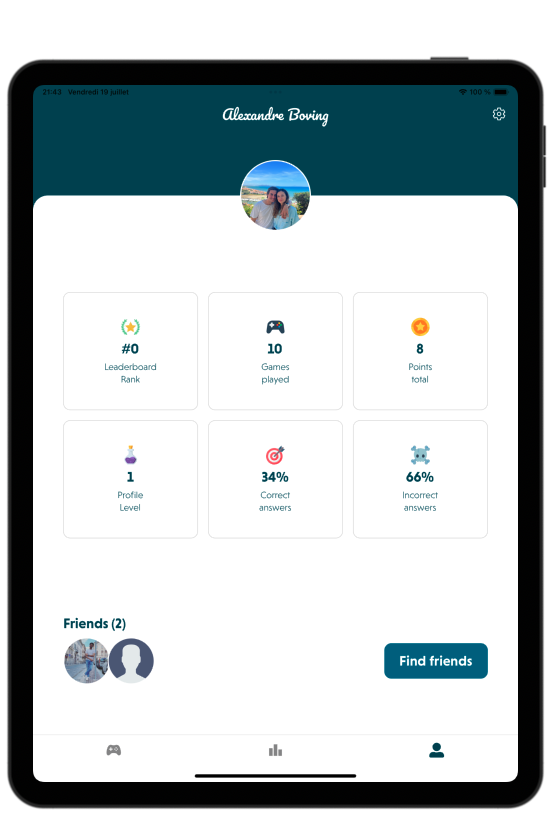
\includegraphics[width=\linewidth]{TabletUI/User Profile UI with Statistics.png}
        \caption{\textbf{User Profile UI with Statistics}}
    \end{minipage}
\end{figure}


The Profile Page offers a comprehensive overview of the user's achievements and statistics within the BrainMe application. At the top, users can see their profile picture and username, providing a personalized touch. Below this, various statistics and achievements are displayed, including:

\begin{itemize}
\item \textbf{Leaderboard Rank:} Shows the user's current rank on the leaderboard, motivating them to improve their performance.
\item \textbf{Games Played:} Displays the total number of games the user has participated in.
\item \textbf{Points Total:} Indicates the total points accumulated by the user.
\item \textbf{Profile Level:} Represents the user's profile level based on their activity and achievements.
\item \textbf{Correct Answers:} Shows the percentage of questions the user has answered correctly.
\item \textbf{Incorrect Answers:} Displays the percentage of questions the user has answered incorrectly.
\end{itemize}

Additionally, there is a "Find Friends" button that allows users to search for and connect with other users within the app, enhancing the social learning experience. The clean and intuitive design ensures that users can easily access and understand their statistics, fostering a sense of achievement and encouraging continuous engagement with the app.

\subsubsection{Friend list and checking other user's profile}

\begin{figure}[H]
    \centering
    \begin{minipage}[b]{0.43\linewidth}
        \centering
        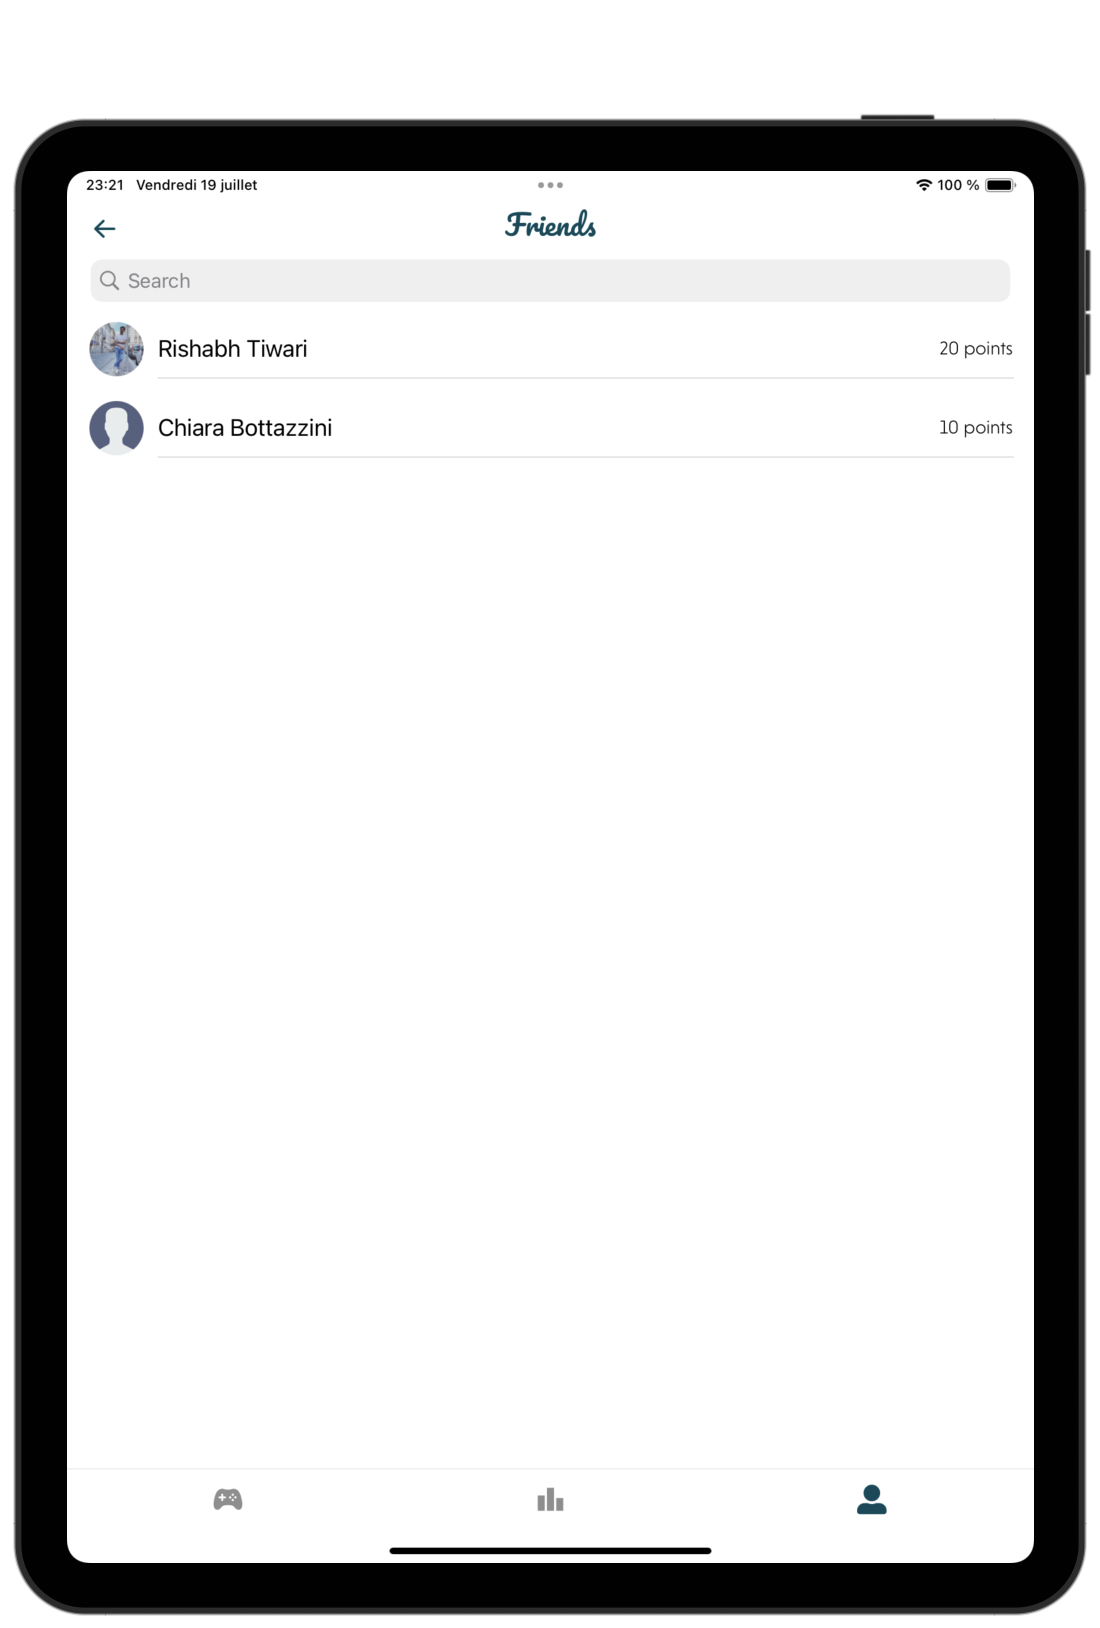
\includegraphics[width=\linewidth]{TabletUI/User's friends list.png}
        \caption{User's friends list}
    \end{minipage}
    \hspace{0.1\linewidth}
    \begin{minipage}[b]{0.43\linewidth}
        \centering
        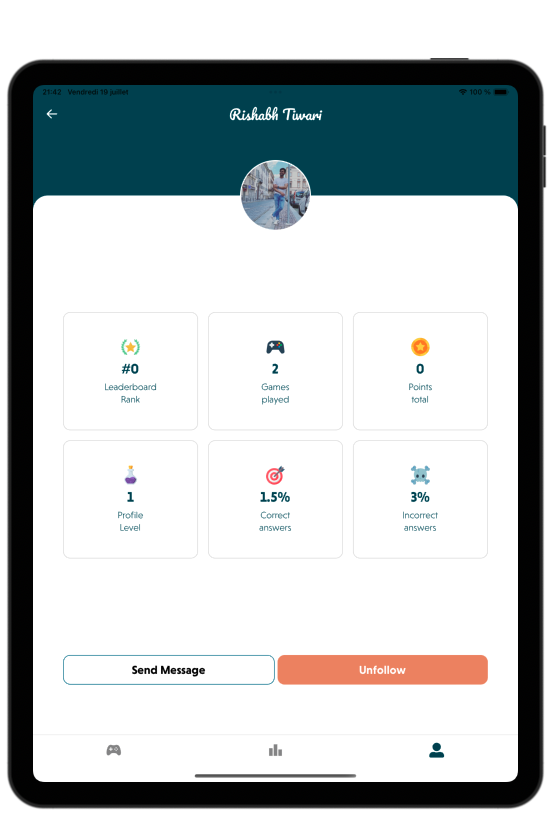
\includegraphics[width=\linewidth]{TabletUI/Friend's User Profile.png}
        \caption{Friend's User Profile}
    \end{minipage}
    \vspace{0.5cm}
    \caption{\textbf{User's friend list along with friend's user profile}}
\end{figure}

The Friend List and Checking Other User's Profile feature in BrainMe enhances the social interaction aspect of the application. It allows users to view the friends they already follow and view their progress and achievements.

\begin{itemize}
\item \textbf{Friend List:} Users can see their friends' names, profile pictures, and the points they have earned. A search bar at the top allows users to quickly find specific friends by name.
\item \textbf{Friend's User Profile:} This shows a friend's detailed profile when selected from the friends list. The profile includes the friend's leaderboard rank, games played, total points, profile level, correct answer percentage, and incorrect answer percentage. Additionally, users can send a message or unfollow the friend using the buttons provided.
\end{itemize}

This feature promotes a competitive and collaborative environment, motivating users to improve their performance by comparing their achievements with those of their friends.

\subsubsection{Find Friends}

\begin{figure}[H]
    \centering
    \begin{minipage}[b]{0.43\linewidth}
        \centering
        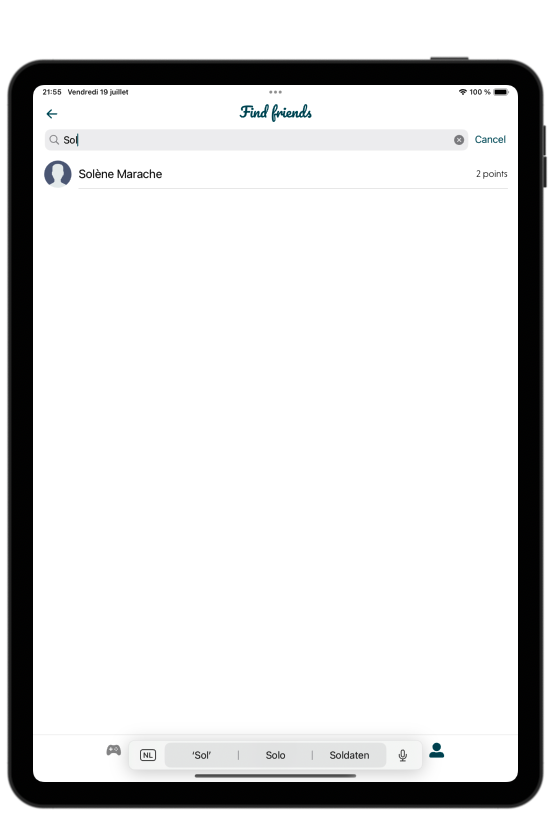
\includegraphics[width=\linewidth]{TabletUI/Searching for a friend from the available users.png}
        \caption{Searching for a friend from the available users}
    \end{minipage}
    \hspace{0.1\linewidth}
    \begin{minipage}[b]{0.43\linewidth}
        \centering
        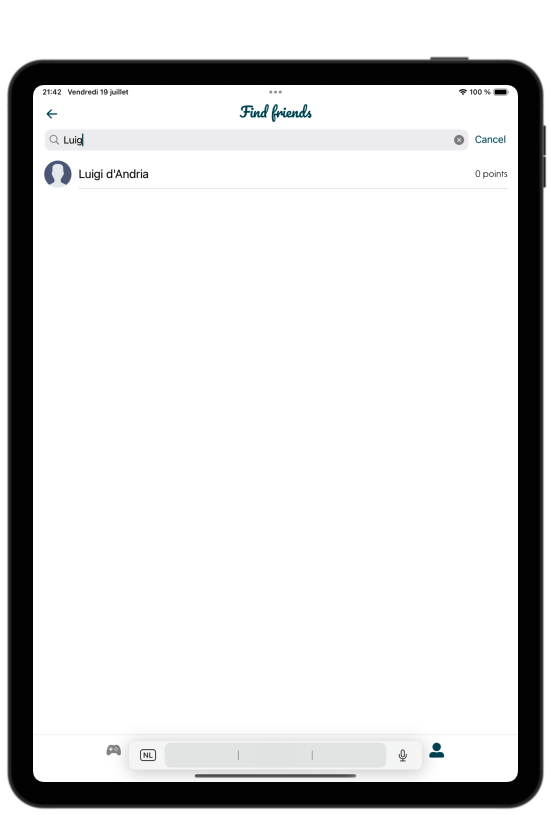
\includegraphics[width=\linewidth]{TabletUI/Filter search for following a friend.png}
        \caption{Filter search for following a friend}
    \end{minipage}
    \vspace{0.5cm}
    \caption{\textbf{User can search for a friend and follow them}}
\end{figure}

The Find Friends feature in BrainMe allows users to search for and connect with other users. This promotes social interaction and collaboration within the application.

\begin{itemize}
\item \textbf{Searching for a Friend:} The left screen shows the user entering a friend's name into the search bar. As the user types, the app filters the list to display matching names. This makes it easy for users to find specific friends quickly.
\item \textbf{Filter Search for Adding:} The right screen displays the results of the search, showing the user’s profile picture, name, and points. Users can select a friend from the list to view their profile and follow them.
\end{itemize}

\subsubsection{Chat Page}

\begin{figure}[H]
    \centering
    \begin{minipage}[b]{0.43\linewidth}
        \centering
        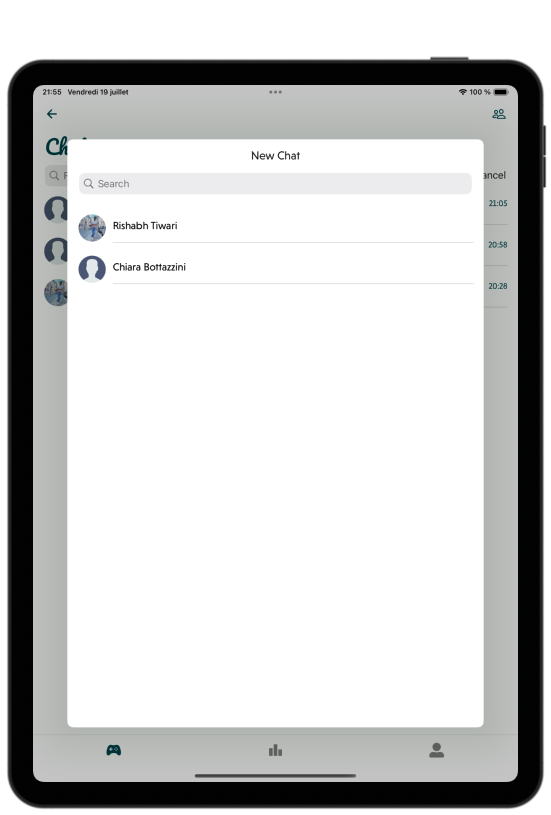
\includegraphics[width=\linewidth]{TabletUI/Creating a new chat.png}
        \caption{Creating new chat}
    \end{minipage}
    \hspace{0.1\linewidth}
    \begin{minipage}[b]{0.43\linewidth}
        \centering
        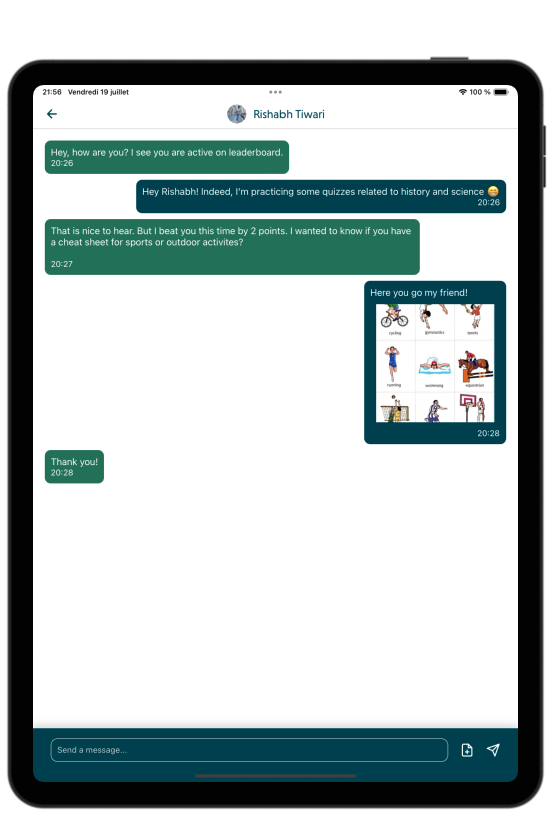
\includegraphics[width=\linewidth]{TabletUI/Chat System Example.png}
        \caption{Chat System Example}
    \end{minipage}
    \vspace{0.5cm}
    \caption{\textbf{Creation and an example of a new chat with file sharing}}
\end{figure}

The chat page allows users to create new chats and engage in conversations with other users. This feature supports both text and file sharing, enhancing the communication experience within the app.

\begin{itemize}
    \item \textbf{Creating New Chat:} Users can easily initiate a new chat with their friends by selecting from a list of contacts.
    \item \textbf{Chat System Example:} The chat interface displays messages exchanged between users, including the time stamps and any shared files.
    \item \textbf{File Sharing:} Users can share images and other files within the chat, making it more interactive and engaging.
\end{itemize}

\subsubsection{Settings Page}

\begin{figure}[H]
    \centering
    \begin{minipage}[b]{0.43\linewidth}
        \centering
        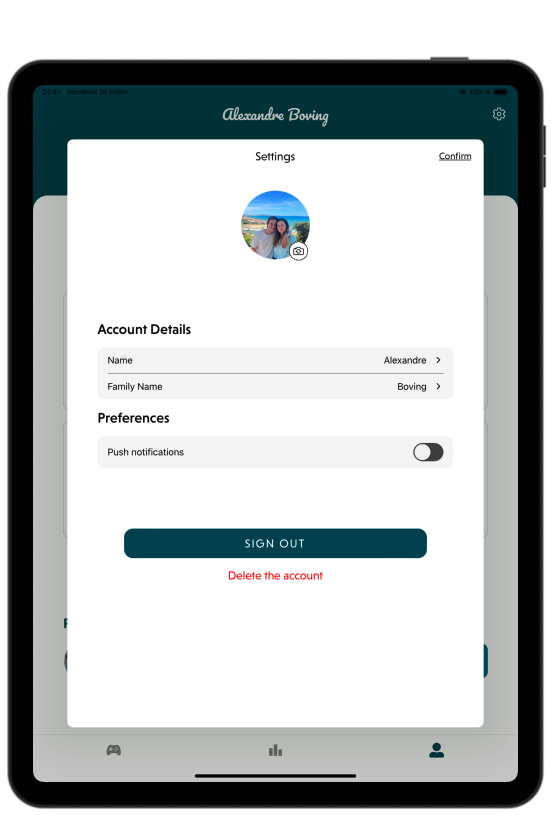
\includegraphics[width=\linewidth]{TabletUI/Account Settings Page.png}
        \caption{Account Settings Page}
    \end{minipage}
    \hspace{0.1\linewidth}
    \begin{minipage}[b]{0.43\linewidth}
        \centering
        \includegraphics[width=\linewidth]{TabletUI/Push Notifications.png}
        \caption{Push Notifications}
    \end{minipage}
    \vspace{0.5cm}
    \caption{\textbf{Account Settings with Push Notifications}}
\end{figure}

The Settings Page in BrainMe provides users with the ability to manage their account details and preferences, ensuring a personalized and secure experience. Users can choose to opt in or opt out of the push notifications and also update their profile image and other personal details.